% !TEX root = Prezentace.tex

\usetheme{default}

\usepackage{colortbl}
\usepackage{xltxtra}
\usepackage{nameref}
\usepackage{tikz, pgf, pgfplots}
\usepackage{gnuplot-lua-tikz}
\makeatletter
\newcommand*{\sectionframe}{\frame{\huge{\textbf{\thesection}. \@currentlabelname}}}
\makeatother
\usepackage[authoryear]{natbib}
\usepackage{rotating}

\title{Lock-chart solving}
\subtitle{Dissertation defense}

\author{Radomír Černoch}
\date{27/6/2018}

\newcommand\cinv{\cellcolor{black}\color{white}}
\newcommand\bigforall{\mbox{\Large $\mathsurround0pt\forall$}}


\begin{document}

\begin{frame}
  \titlepage
\end{frame}



\section{Introduction}
\sectionframe



\begin{frame}{Tumbler lock}
  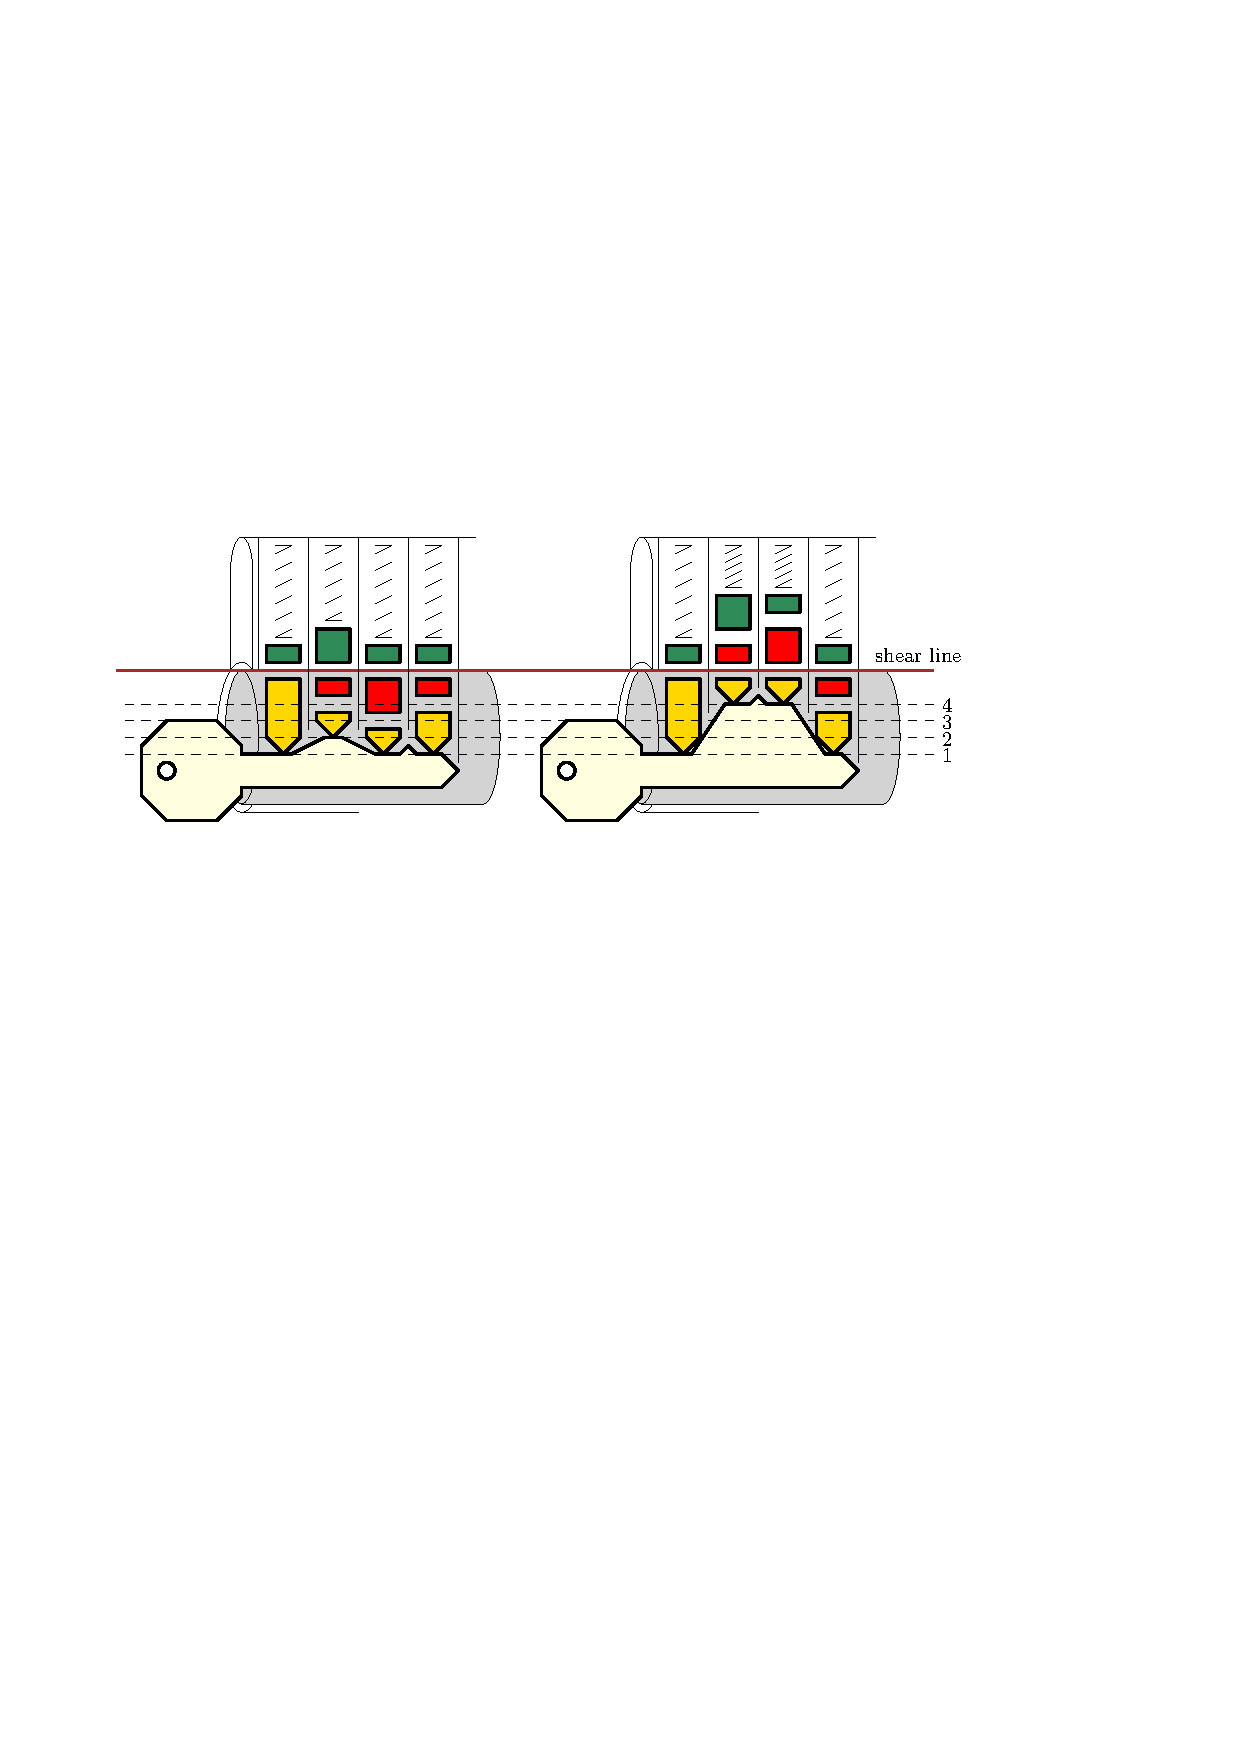
\includegraphics[width=\textwidth]{TumblerLock.pdf}
  \pause
  In this picture:
  \begin{itemize}
    \item There are 4 \emph{positions} (vertical bars).
    \item There are 4 \emph{cutting depths} (horizontal lines).
  \end{itemize}
  $$p=4, d=4$$
\end{frame}

\begin{frame}{Lock-chart problem}
  \begin{minipage}[t][180pt][t]{\textwidth}
    \only<1|handout:0>{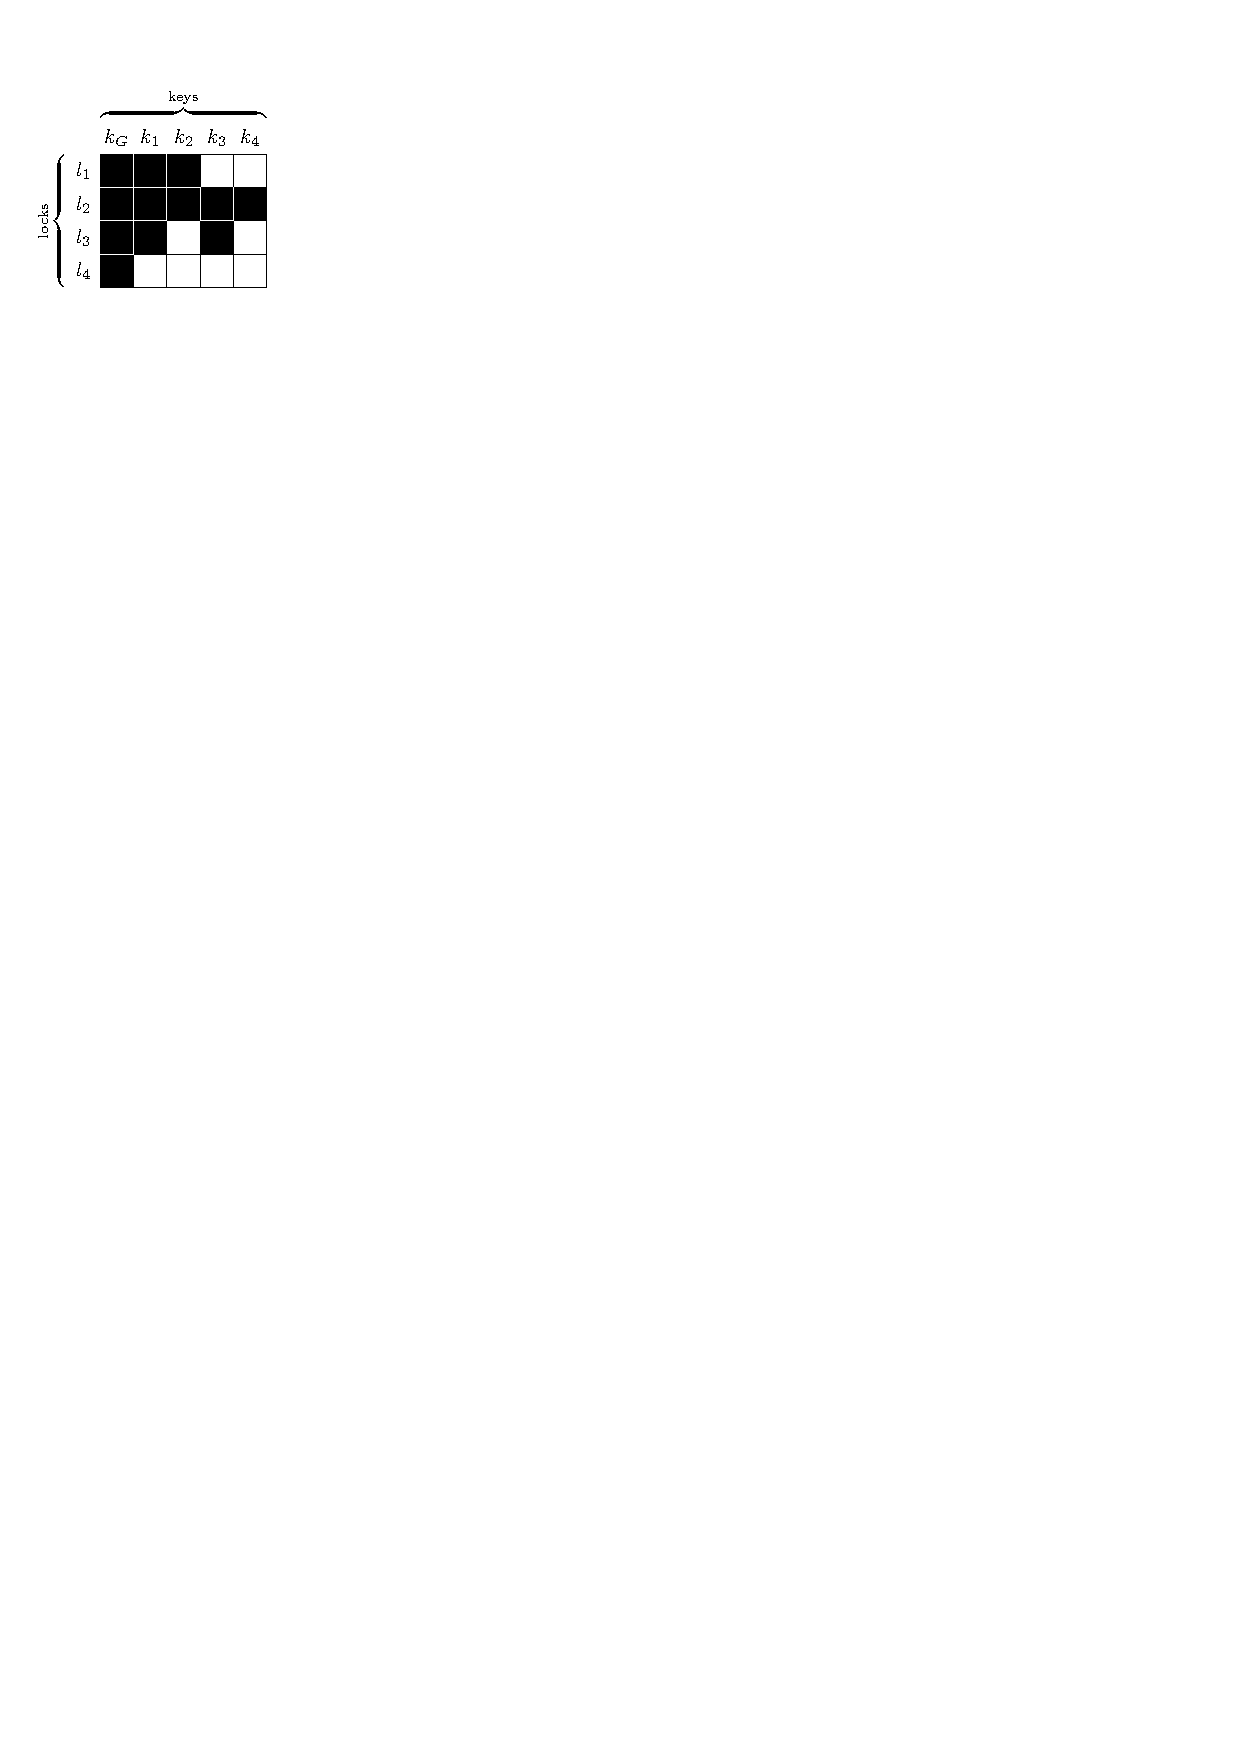
\includegraphics{Definitions1.pdf}}
    \only<2|handout:1>{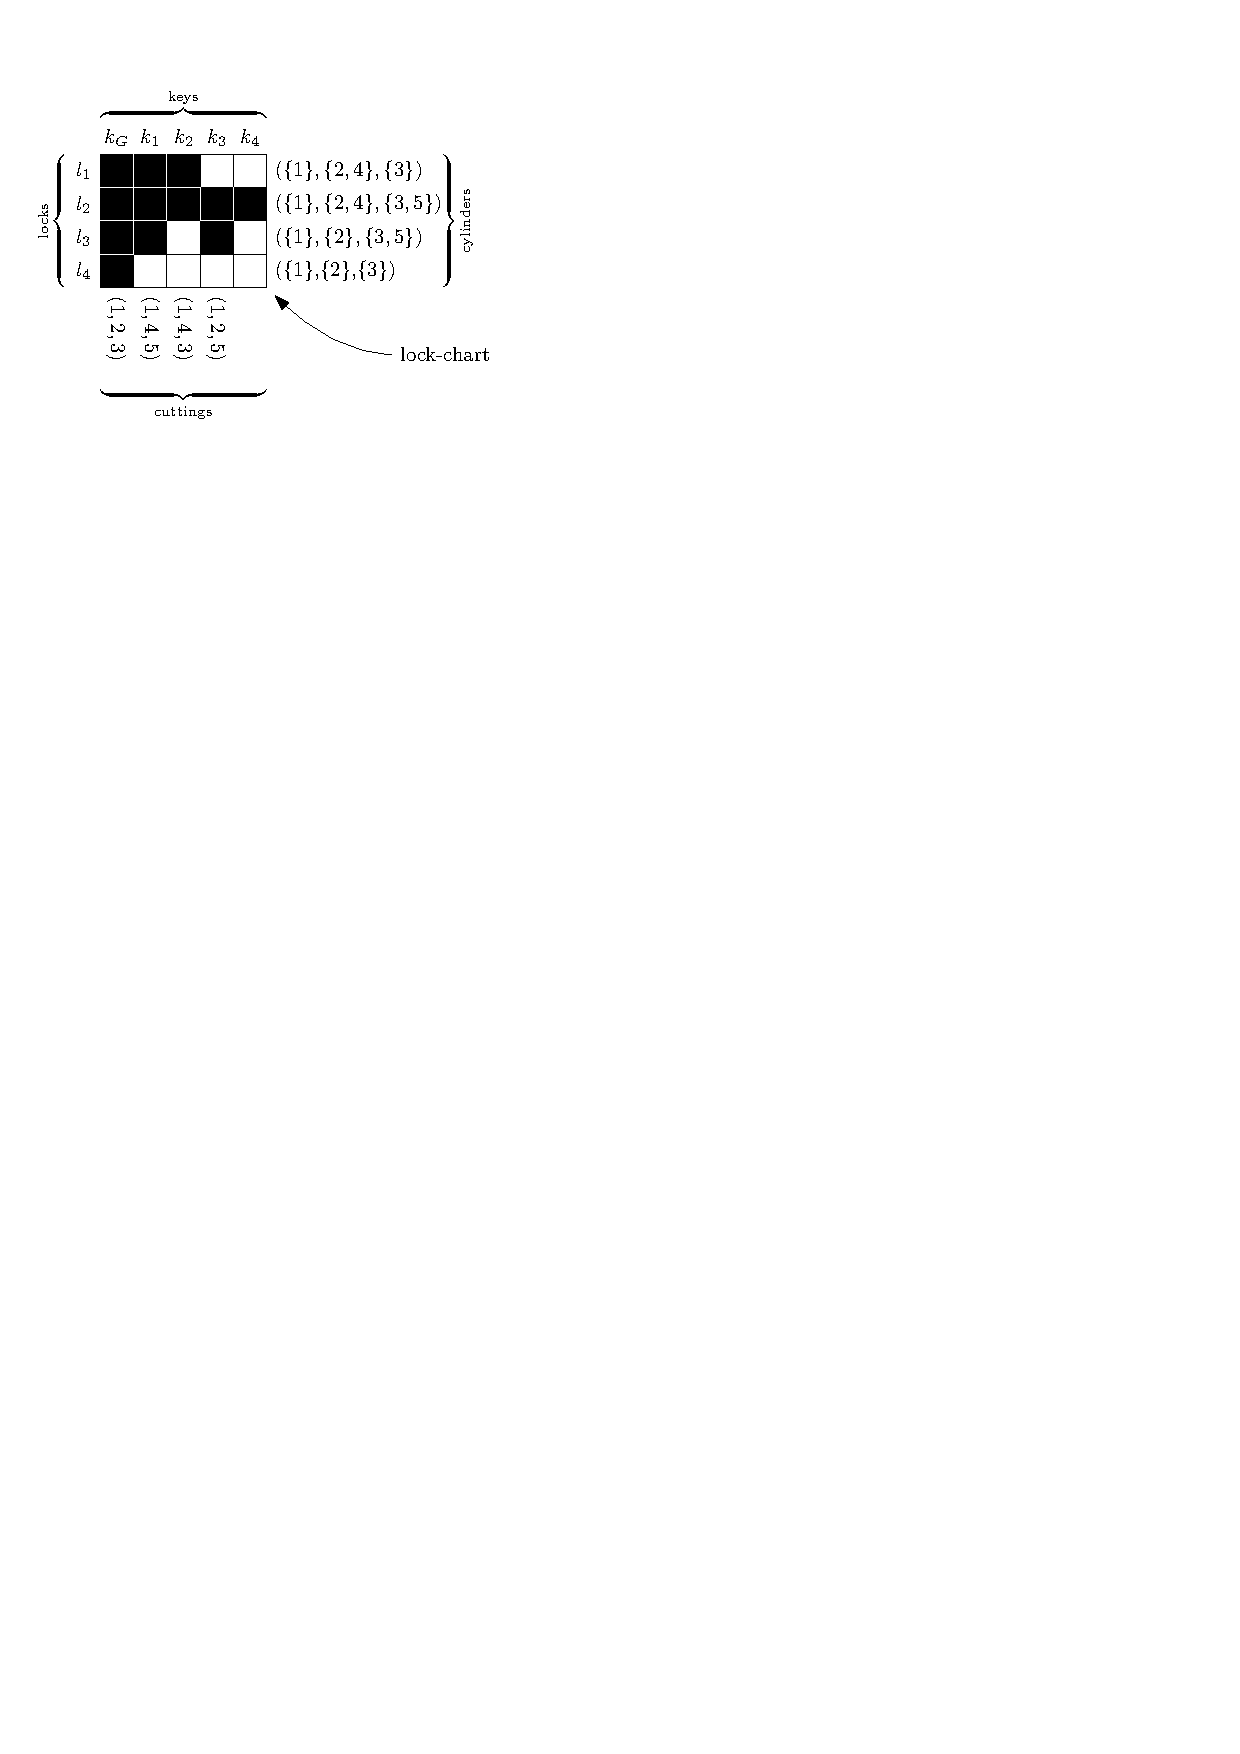
\includegraphics{Definitions2.pdf}}
    %\only<3|handout:1>{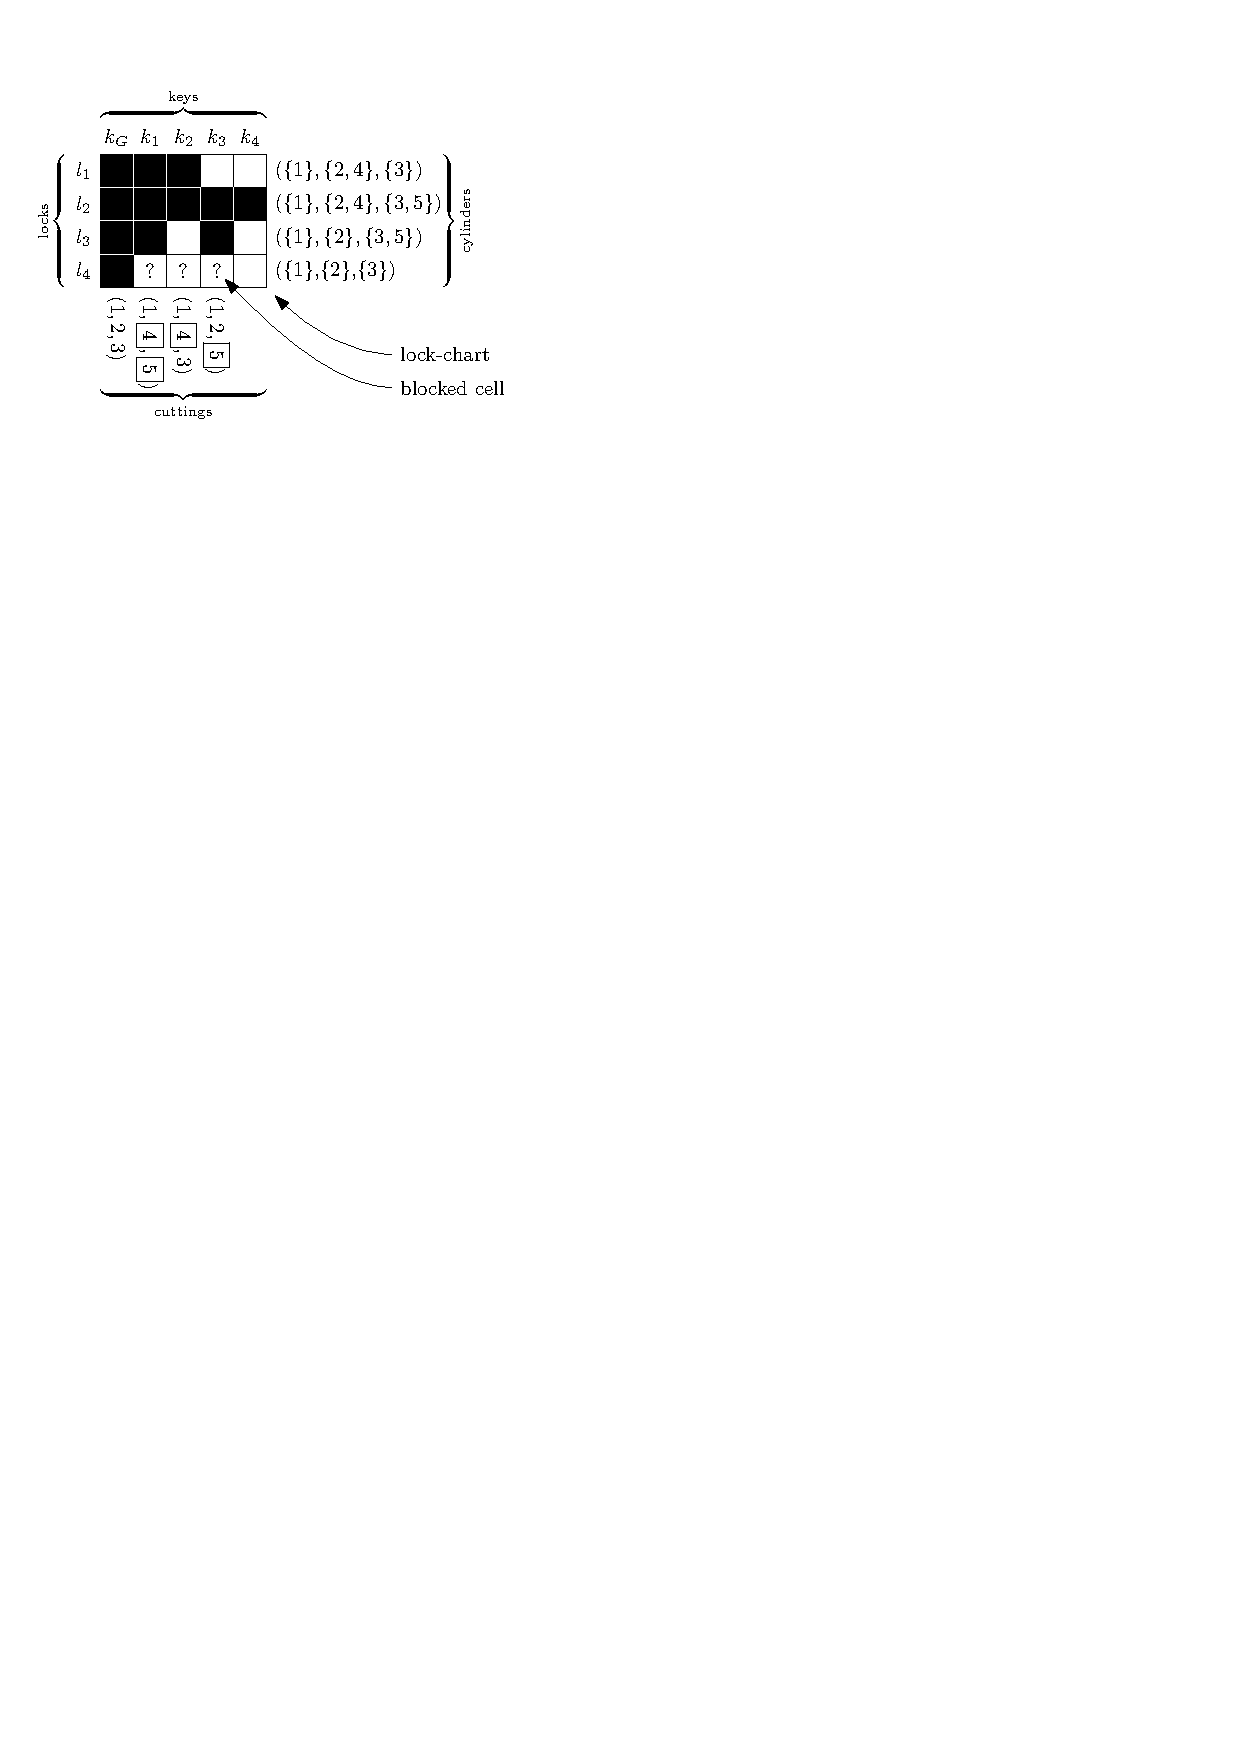
\includegraphics{Definitions3.pdf}}
  \end{minipage}
\end{frame}

\begin{frame}{Motivation}
  \begin{block}{Reviewer's comment}
    Based on the presented research,
    has there been a progamme written
    that could be practically used
    to design master keyed systems?
  \end{block}
  \begin{block}{Otázka oponenta}
    Byl na základě představeného výzkumu napsán program,
    který se v praxi použil na návrh zámků a klíčů,
    případně na nějaké dílčí úlohy?
  \end{block}
\end{frame}


\begin{frame}{Motivation}
  \begin{minipage}[t][180pt][t]{.40\textwidth}
    \bigskip

    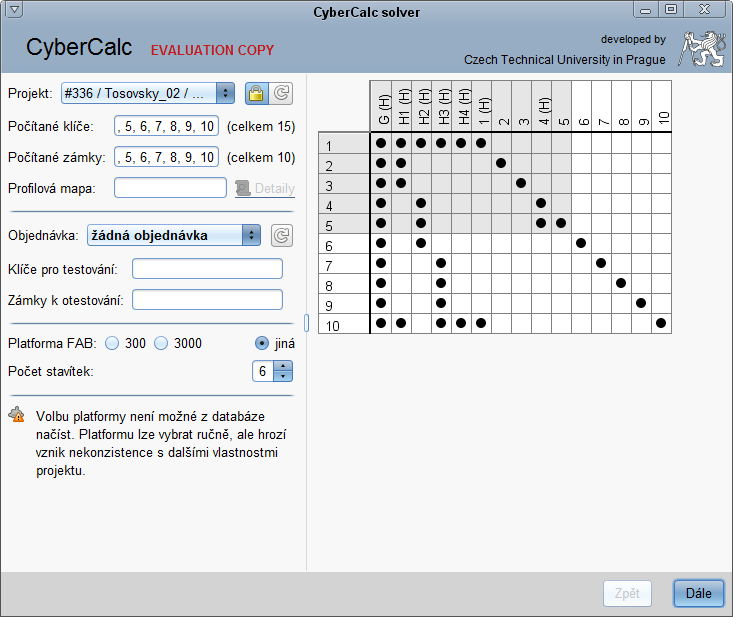
\includegraphics[width=\textwidth]{Extension.png}
  \end{minipage}
  \pause
  \hfill
  \begin{minipage}[t][180pt][t]{.55\textwidth}
    \textbf{CyberCalc:} Depth-first-search with
    constraint-satisfaction pruning 
    and many heuristics.

    \pause

    \begin{block}{Issues}
      \begin{itemize}
        \item \textbf{Lack of insight} into heuristics' effects.
        \item Does not scale for \textbf{modern platforms} with $\geq 10^6$ key cuttings. 
        \item Can some subproblems be \textbf{polynomial}? Under which assumptions?
        \item The \textbf{extensibility} problem.
      \end{itemize}
    \end{block}
  \end{minipage}
\end{frame}


\begin{frame}{Motivation}
  \begin{center}
    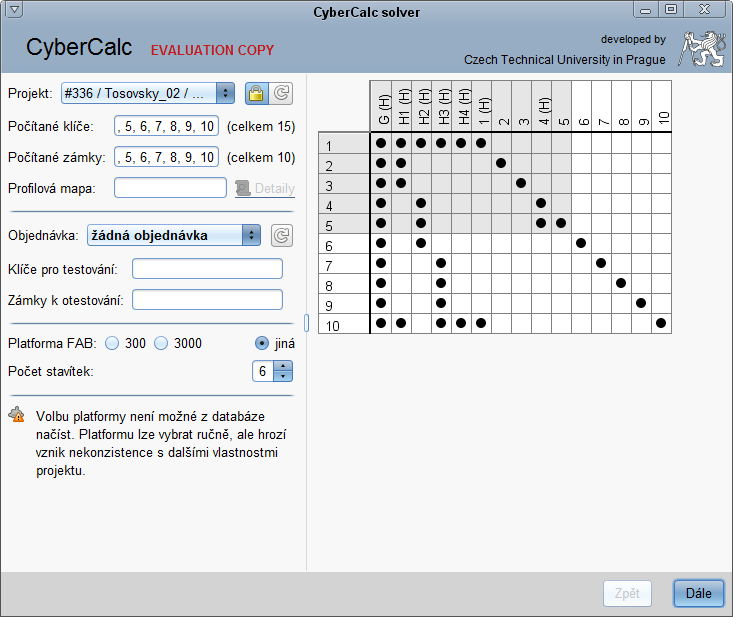
\includegraphics[width=\textwidth]{Extension.png}
  \end{center}
\end{frame}



\section{Complexity classes}
\sectionframe



\begin{frame}{Frameworks}
  4 constraint \textit{frameworks} of increasing expressivity:
  \begin{enumerate}
    \item \textbf{Vanilla}: Number of positions $p$ and cutting depths $d$.
    \item (\textbf{Asymmetric}: Number of cutting depths varies between positions.)
    \item \textbf{General}: Plus a set of \textit{general constraints} (gecons).
    \item (\textbf{Explicit}: List of valid key cuttings is algorithm's input.)
  \end{enumerate}
\end{frame}

\begin{frame}{General framework}
  \begin{minipage}[t][180pt][t]{.4\textwidth}
    \bigskip

    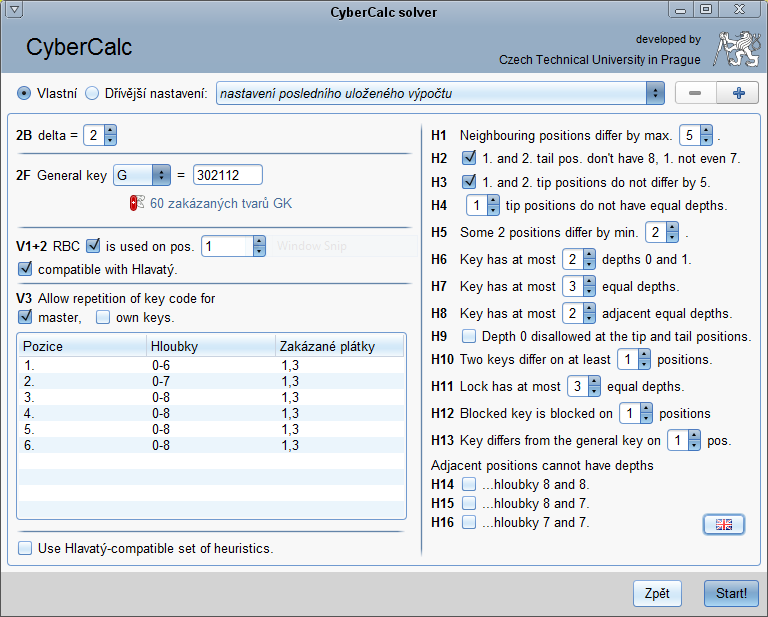
\includegraphics[width=\textwidth]{Constraints.png}
  \end{minipage}
  \begin{minipage}[t][180pt][t]{.55\textwidth}
    \begin{block}{Why gecons?}
      \begin{itemize}
        \item Most constraints “overlap”, \textbf{counting key cuttings} that satisfy all constraints is difficult.
        \item \textbf{Gecon} = a formally defined group of forbidden key cuttings.
        \item 15 rules can be each “compiled” to a set of gecons.
      \end{itemize}
    \end{block}
  \end{minipage}
\end{frame}

\begin{frame}{General framework}
  \begin{minipage}[t][180pt][t]{.40\textwidth}
    \bigskip

    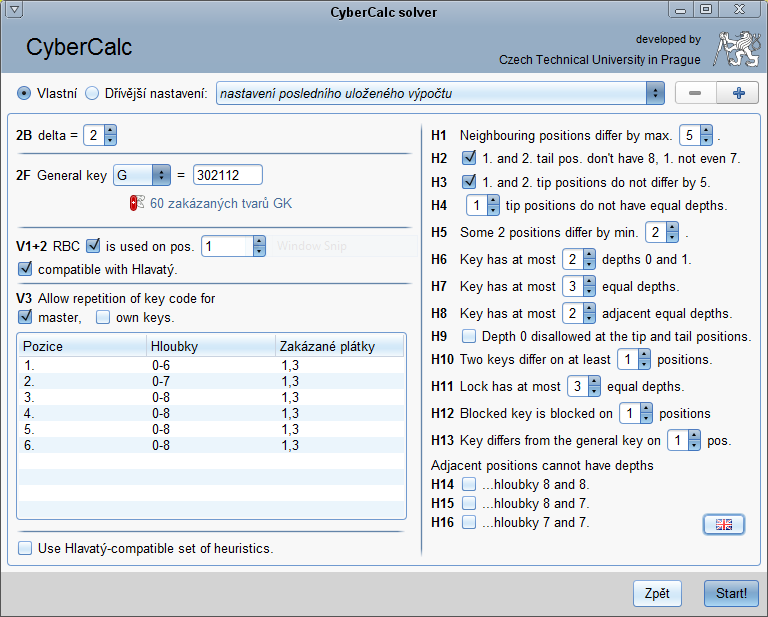
\includegraphics[width=\textwidth]{Constraints.png}
  \end{minipage}
  \begin{minipage}[t][180pt][t]{.55\textwidth}
    \begin{block}{Counting key cuttings}
      \begin{itemize}
        \item Derive number of key cuttings \textbf{invalidated} by 1 gecon.
        \item Define an \textbf{intersection} of 2 gecons (which is also a gecon).
        \item Design a \textbf{inclusion-exclusion} counting procedure.
        \item It can count $\approx 840 \cdot 10^6$ keys within $60\,$s.
      \end{itemize}
    \end{block}
  \end{minipage}
\end{frame}

\begin{frame}{General framework}
  \begin{block}{$\mathcal{NP}$-completeness}
    \begin{itemize}
      \item \textbf{Gecon} corresponds to 1 clause in the SAT problem.
      \item SAT is equivalent to solving a
            “$1 \text{ key} \times 0 \text{ locks}$” lock-chart.
      \item Lock-chart solving in the general framework is $\mathcal{NP}$-complete.
    \end{itemize}
  \end{block}
  \pause
  \begin{block}{Counting key cuttings}
    \begin{itemize}
      \item Both reductions \textbf{preserve} the number of solutions.
      \item \#SAT counts the number of valid key cuttings.
      \item Counting key cuttings is in $\#\mathcal{P}$.
    \end{itemize}
  \end{block}
\end{frame}

\begin{frame}{$\mathcal{NP}$-complete classes}
  $\bullet$ = lock-chart problem instance grows in this parameter

  \vfill
  \begin{tabular}{r|cc|ccc|ccl}
       & framework & lock-chart      & \begin{rotate}{60}positions\end{rotate} & \begin{rotate}{60}depths\end{rotate} & \begin{rotate}{60}gecons\end{rotate} & \begin{rotate}{60}keys\end{rotate} & \begin{rotate}{60}locks\end{rotate} &                  \\\hline
    1. & general   & all             & $\bullet$                               &                                      & $\bullet$                            &                                    &                                     &                  \\\pause
    2. & vanilla   & extension       & $\bullet$                               &                                      &                                      &                                    & $\bullet$                           & \cite{lawer2004} \\\pause
    3. & vanilla   & melted-profiles &                                         & $\bullet$                            &                                      & $\bullet$                          & $\bullet$                           &                  \\
  \end{tabular}

  \vfill
  \begin{itemize}
    \item Results 1. and 2. proved by a reduction from SAT.
    \item Result 3. by a reduction from \textit{k}-coloring.
  \end{itemize}
\end{frame}


\begin{frame}{Vanilla framework}
  Complexity classes of lock-chart problem variants:
  \begin{center}
    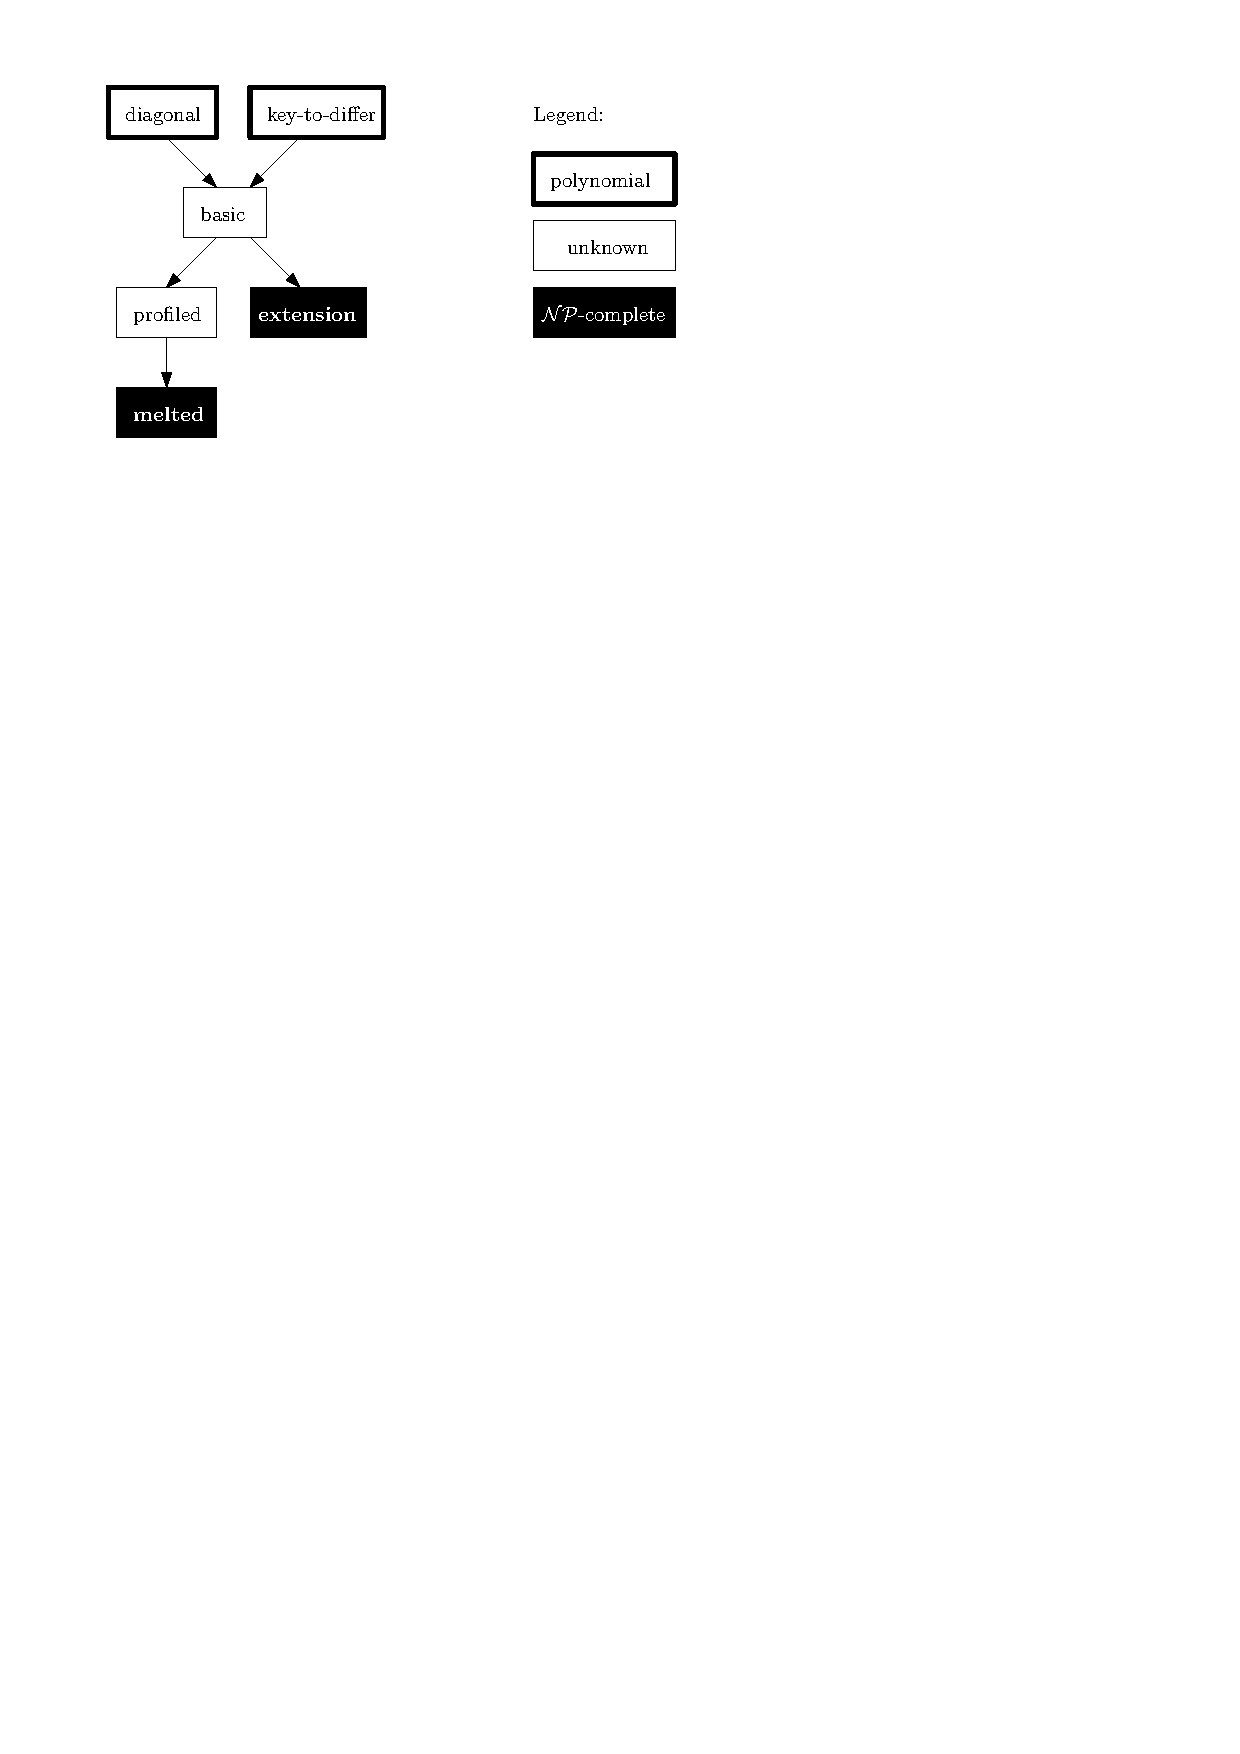
\includegraphics[width=.7\textwidth]{LockChartHierarchy.pdf}  
  \end{center}
\end{frame}



\begin{frame}{Vanilla framework}
  \begin{minipage}[t][180pt][t]{.45\textwidth}
    \emph{Diagonal} lock-chart:

    \bigskip

    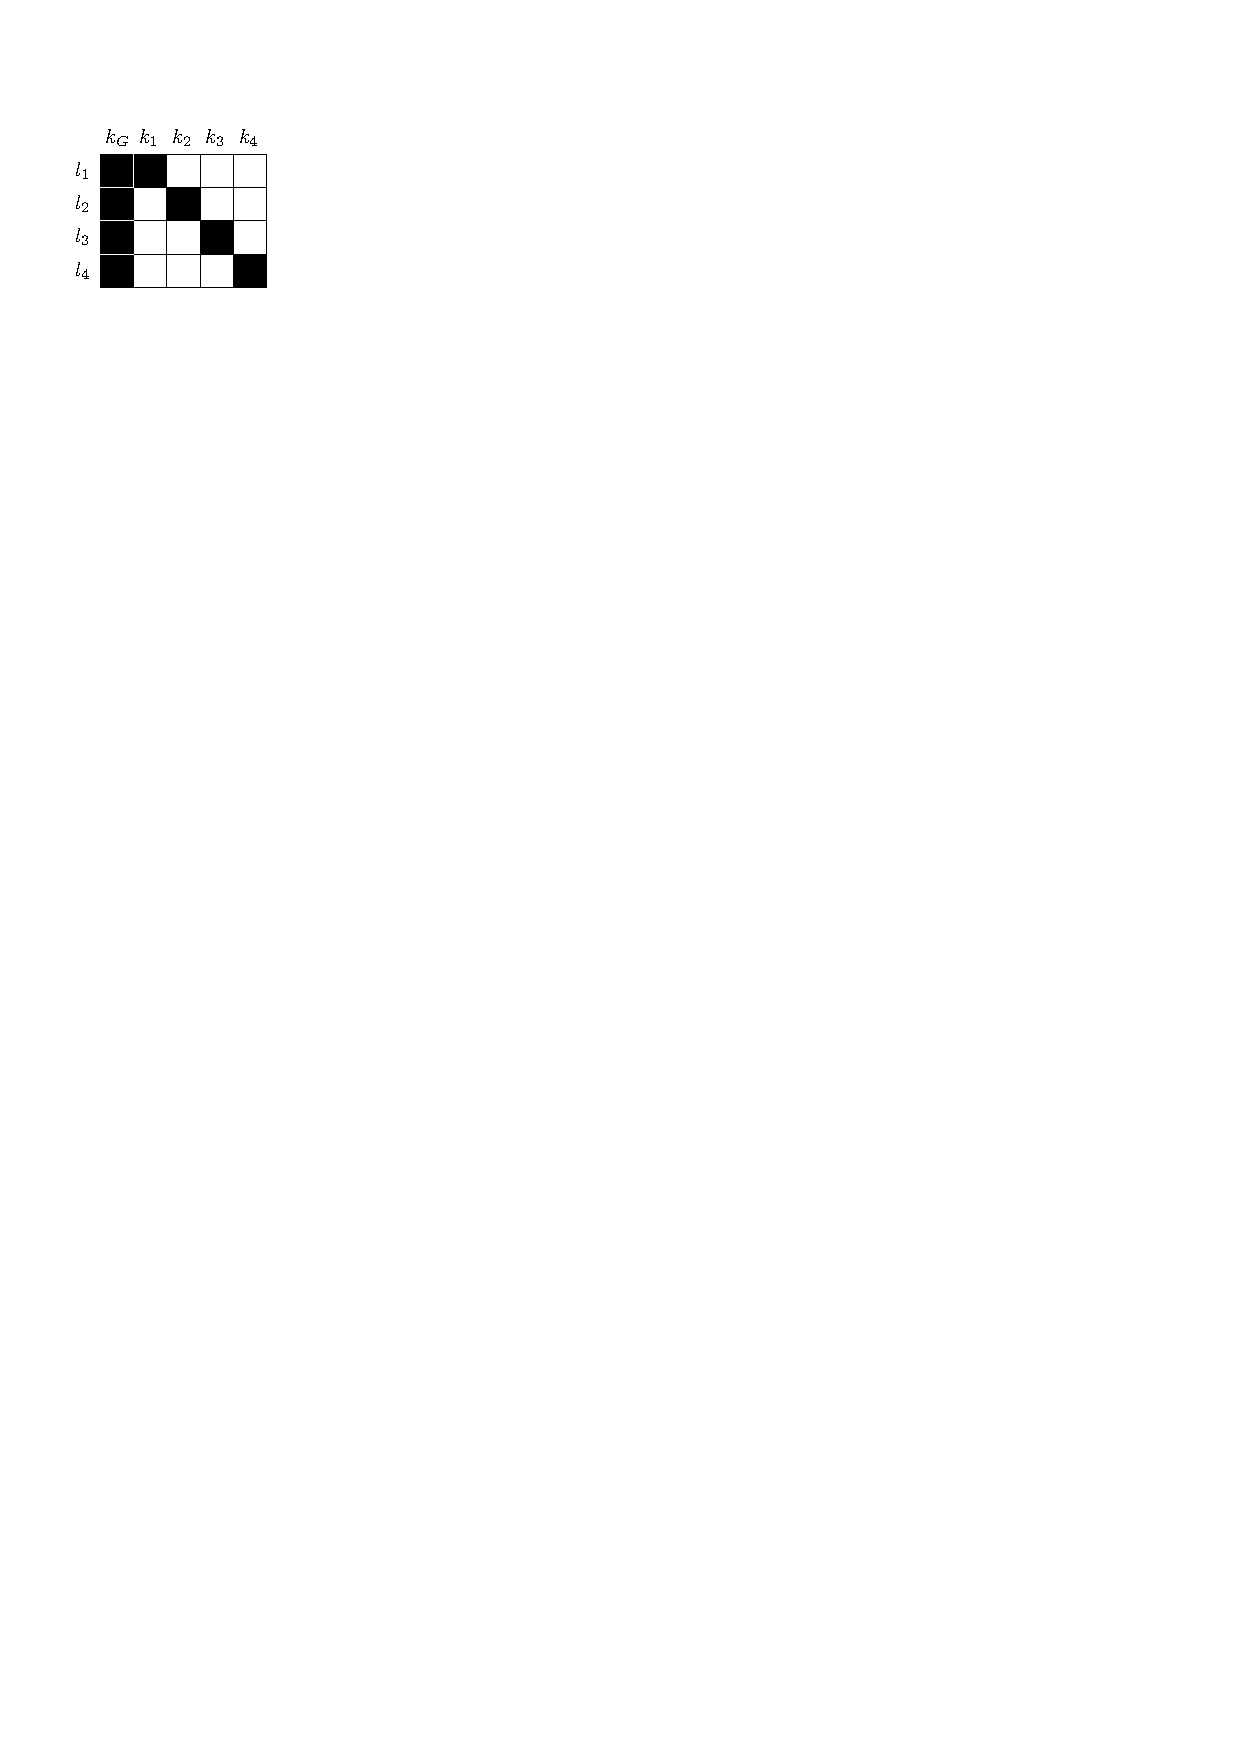
\includegraphics{DiagonalLockChart.pdf}

    Contains exactly 1 \emph{general} key which opens all locks
    and several \emph{individual} keys which open exactly 1 lock.
  \end{minipage}
  \pause
  \hfill
  \begin{minipage}[t][180pt][t]{.45\textwidth}
    \begin{block}{Properties}
      \begin{itemize}
        \item Finding cuttings for individual keys translates to the
        \textit{maximum independent set} (MIS) problem.
        \item This is true for all frameworks.
      \end{itemize}
    \end{block}
  \end{minipage}
\end{frame}

\begin{frame}{Vanilla framework}
  \begin{block}{Structure of the MIS graph}
    \begin{itemize}
      \item The MIS graph can be partitioned into $S_0, \ldots, S_p$ \textbf{classes},
        based on the distance to the cutting of the general key.
      \item Size of the $q$-th class was derived to be
        $$|S_q| = \binom{p}{p-q}\cdot (d-1)^{p-q}\ ,$$
        maximized if $q=\hat q$, where
        $$\hat{q}=\left\lfloor \frac{p+1}{d}\right\rfloor\ .$$
      \pause
      \item Each $S_q$ class is an independent set (true in every fw.).
      \item $S_{\hat{q}}$ is the maximum independent set (in vanilla fw.).
      \pause
      \item The \textit{rotating constant method} (RCM) was analysed.
    \end{itemize}
  \end{block}
\end{frame}

\begin{frame}{Vanilla framework}
  \begin{itemize}
    \item Solution exists iff the number of keys is at most $|S_{\hat{q}}|$.
    \item Diagonal lock-charts in the vanilla framework are polynomial.
  \end{itemize}
\end{frame}


\begin{frame}{Other frameworks}
  \begin{itemize}
    \item MIS is $\mathcal{NP}$-complete, but it can be approximated.
    \pause
    \item Since each $S_q$ is an independent set,
      RCM gives at least a \textbf{lower bound} on the MIS size.
    \item How tight is this bound?
  \end{itemize}
\end{frame}

\begin{frame}{Other frameworks}
  \begin{minipage}[t][180pt][t]{.44\textwidth}
    \begin{itemize}
      \item Real-world constraints were randomly sampled.
      \item The MIS graph was constructed in memory.
      \item RCM was compared againts an exact algorithm\\
        (backtracking, exponential runtime).
    \end{itemize}
  \end{minipage}
  \hfill
  \begin{minipage}[t][180pt][t]{.45\textwidth}
    \bigskip

    \resizebox{1.1\textwidth}{1.1\textwidth}{%
      \begin{tikzpicture}[gnuplot][scale=0.50]
%% generated with GNUPLOT 5.0p5 (Lua 5.1; terminal rev. 99, script rev. 102)
%% Fri 01 Jun 2018 10:56:14 AM DST
\path (0.000,0.000) rectangle (10.000,10.000);
\gpcolor{color=gp lt color axes}
\gpsetlinetype{gp lt axes}
\gpsetdashtype{gp dt axes}
\gpsetlinewidth{0.50}
\draw[gp path] (1.136,0.985)--(9.447,0.985);
\gpcolor{color=gp lt color border}
\gpsetlinetype{gp lt border}
\gpsetdashtype{gp dt solid}
\gpsetlinewidth{1.00}
\draw[gp path] (1.136,0.985)--(1.316,0.985);
\draw[gp path] (9.447,0.985)--(9.267,0.985);
\node[gp node right] at (0.952,0.985) {$0$};
\gpcolor{color=gp lt color axes}
\gpsetlinetype{gp lt axes}
\gpsetdashtype{gp dt axes}
\gpsetlinewidth{0.50}
\draw[gp path] (1.136,2.714)--(9.447,2.714);
\gpcolor{color=gp lt color border}
\gpsetlinetype{gp lt border}
\gpsetdashtype{gp dt solid}
\gpsetlinewidth{1.00}
\draw[gp path] (1.136,2.714)--(1.316,2.714);
\draw[gp path] (9.447,2.714)--(9.267,2.714);
\node[gp node right] at (0.952,2.714) {$10$};
\gpcolor{color=gp lt color axes}
\gpsetlinetype{gp lt axes}
\gpsetdashtype{gp dt axes}
\gpsetlinewidth{0.50}
\draw[gp path] (1.136,4.443)--(9.447,4.443);
\gpcolor{color=gp lt color border}
\gpsetlinetype{gp lt border}
\gpsetdashtype{gp dt solid}
\gpsetlinewidth{1.00}
\draw[gp path] (1.136,4.443)--(1.316,4.443);
\draw[gp path] (9.447,4.443)--(9.267,4.443);
\node[gp node right] at (0.952,4.443) {$20$};
\gpcolor{color=gp lt color axes}
\gpsetlinetype{gp lt axes}
\gpsetdashtype{gp dt axes}
\gpsetlinewidth{0.50}
\draw[gp path] (1.136,6.173)--(9.447,6.173);
\gpcolor{color=gp lt color border}
\gpsetlinetype{gp lt border}
\gpsetdashtype{gp dt solid}
\gpsetlinewidth{1.00}
\draw[gp path] (1.136,6.173)--(1.316,6.173);
\draw[gp path] (9.447,6.173)--(9.267,6.173);
\node[gp node right] at (0.952,6.173) {$30$};
\gpcolor{color=gp lt color axes}
\gpsetlinetype{gp lt axes}
\gpsetdashtype{gp dt axes}
\gpsetlinewidth{0.50}
\draw[gp path] (1.136,7.902)--(9.447,7.902);
\gpcolor{color=gp lt color border}
\gpsetlinetype{gp lt border}
\gpsetdashtype{gp dt solid}
\gpsetlinewidth{1.00}
\draw[gp path] (1.136,7.902)--(1.316,7.902);
\draw[gp path] (9.447,7.902)--(9.267,7.902);
\node[gp node right] at (0.952,7.902) {$40$};
\gpcolor{color=gp lt color axes}
\gpsetlinetype{gp lt axes}
\gpsetdashtype{gp dt axes}
\gpsetlinewidth{0.50}
\draw[gp path] (1.136,9.631)--(9.447,9.631);
\gpcolor{color=gp lt color border}
\gpsetlinetype{gp lt border}
\gpsetdashtype{gp dt solid}
\gpsetlinewidth{1.00}
\draw[gp path] (1.136,9.631)--(1.316,9.631);
\draw[gp path] (9.447,9.631)--(9.267,9.631);
\node[gp node right] at (0.952,9.631) {$50$};
\gpcolor{color=gp lt color axes}
\gpsetlinetype{gp lt axes}
\gpsetdashtype{gp dt axes}
\gpsetlinewidth{0.50}
\draw[gp path] (1.136,0.985)--(1.136,9.631);
\gpcolor{color=gp lt color border}
\gpsetlinetype{gp lt border}
\gpsetdashtype{gp dt solid}
\gpsetlinewidth{1.00}
\draw[gp path] (1.136,0.985)--(1.136,1.165);
\draw[gp path] (1.136,9.631)--(1.136,9.451);
\node[gp node center] at (1.136,0.677) {$0$};
\gpcolor{color=gp lt color axes}
\gpsetlinetype{gp lt axes}
\gpsetdashtype{gp dt axes}
\gpsetlinewidth{0.50}
\draw[gp path] (2.798,0.985)--(2.798,9.631);
\gpcolor{color=gp lt color border}
\gpsetlinetype{gp lt border}
\gpsetdashtype{gp dt solid}
\gpsetlinewidth{1.00}
\draw[gp path] (2.798,0.985)--(2.798,1.165);
\draw[gp path] (2.798,9.631)--(2.798,9.451);
\node[gp node center] at (2.798,0.677) {$10$};
\gpcolor{color=gp lt color axes}
\gpsetlinetype{gp lt axes}
\gpsetdashtype{gp dt axes}
\gpsetlinewidth{0.50}
\draw[gp path] (4.460,0.985)--(4.460,9.631);
\gpcolor{color=gp lt color border}
\gpsetlinetype{gp lt border}
\gpsetdashtype{gp dt solid}
\gpsetlinewidth{1.00}
\draw[gp path] (4.460,0.985)--(4.460,1.165);
\draw[gp path] (4.460,9.631)--(4.460,9.451);
\node[gp node center] at (4.460,0.677) {$20$};
\gpcolor{color=gp lt color axes}
\gpsetlinetype{gp lt axes}
\gpsetdashtype{gp dt axes}
\gpsetlinewidth{0.50}
\draw[gp path] (6.123,0.985)--(6.123,9.631);
\gpcolor{color=gp lt color border}
\gpsetlinetype{gp lt border}
\gpsetdashtype{gp dt solid}
\gpsetlinewidth{1.00}
\draw[gp path] (6.123,0.985)--(6.123,1.165);
\draw[gp path] (6.123,9.631)--(6.123,9.451);
\node[gp node center] at (6.123,0.677) {$30$};
\gpcolor{color=gp lt color axes}
\gpsetlinetype{gp lt axes}
\gpsetdashtype{gp dt axes}
\gpsetlinewidth{0.50}
\draw[gp path] (7.785,0.985)--(7.785,9.631);
\gpcolor{color=gp lt color border}
\gpsetlinetype{gp lt border}
\gpsetdashtype{gp dt solid}
\gpsetlinewidth{1.00}
\draw[gp path] (7.785,0.985)--(7.785,1.165);
\draw[gp path] (7.785,9.631)--(7.785,9.451);
\node[gp node center] at (7.785,0.677) {$40$};
\gpcolor{color=gp lt color axes}
\gpsetlinetype{gp lt axes}
\gpsetdashtype{gp dt axes}
\gpsetlinewidth{0.50}
\draw[gp path] (9.447,0.985)--(9.447,9.631);
\gpcolor{color=gp lt color border}
\gpsetlinetype{gp lt border}
\gpsetdashtype{gp dt solid}
\gpsetlinewidth{1.00}
\draw[gp path] (9.447,0.985)--(9.447,1.165);
\draw[gp path] (9.447,9.631)--(9.447,9.451);
\node[gp node center] at (9.447,0.677) {$50$};
\draw[gp path] (1.136,9.631)--(1.136,0.985)--(9.447,0.985)--(9.447,9.631)--cycle;
\node[gp node center,rotate=-270] at (0.246,5.308) {RCM};
\node[gp node center] at (5.291,0.215) {exact};
\gpcolor{rgb color={0.000,0.000,0.000}}
\draw[gp path,opacity=0.133] (1.136,0.985)--(1.220,1.422)--(1.304,1.858)--(1.388,2.295)--(1.472,2.732)%
  --(1.556,3.168)--(1.640,3.605)--(1.724,4.042)--(1.808,4.478)--(1.892,4.915)--(1.975,5.352)%
  --(2.059,5.788)--(2.143,6.225)--(2.227,6.662)--(2.311,7.098)--(2.395,7.535)--(2.479,7.972)%
  --(2.563,8.408)--(2.647,8.845)--(2.731,9.282)--(2.798,9.631);
\draw[gp path,opacity=0.133] (1.136,0.985)--(1.220,1.203)--(1.304,1.422)--(1.388,1.640)--(1.472,1.858)%
  --(1.556,2.077)--(1.640,2.295)--(1.724,2.513)--(1.808,2.732)--(1.892,2.950)--(1.975,3.168)%
  --(2.059,3.387)--(2.143,3.605)--(2.227,3.823)--(2.311,4.042)--(2.395,4.260)--(2.479,4.478)%
  --(2.563,4.697)--(2.647,4.915)--(2.731,5.133)--(2.815,5.352)--(2.899,5.570)--(2.983,5.788)%
  --(3.067,6.007)--(3.151,6.225)--(3.235,6.443)--(3.319,6.662)--(3.403,6.880)--(3.487,7.098)%
  --(3.571,7.317)--(3.654,7.535)--(3.738,7.753)--(3.822,7.972)--(3.906,8.190)--(3.990,8.408)%
  --(4.074,8.627)--(4.158,8.845)--(4.242,9.063)--(4.326,9.282)--(4.410,9.500)--(4.460,9.631);
\draw[gp path,opacity=0.133] (1.136,0.985)--(1.220,1.131)--(1.304,1.276)--(1.388,1.422)--(1.472,1.567)%
  --(1.556,1.713)--(1.640,1.858)--(1.724,2.004)--(1.808,2.149)--(1.892,2.295)--(1.975,2.441)%
  --(2.059,2.586)--(2.143,2.732)--(2.227,2.877)--(2.311,3.023)--(2.395,3.168)--(2.479,3.314)%
  --(2.563,3.459)--(2.647,3.605)--(2.731,3.751)--(2.815,3.896)--(2.899,4.042)--(2.983,4.187)%
  --(3.067,4.333)--(3.151,4.478)--(3.235,4.624)--(3.319,4.769)--(3.403,4.915)--(3.487,5.061)%
  --(3.571,5.206)--(3.654,5.352)--(3.738,5.497)--(3.822,5.643)--(3.906,5.788)--(3.990,5.934)%
  --(4.074,6.079)--(4.158,6.225)--(4.242,6.371)--(4.326,6.516)--(4.410,6.662)--(4.494,6.807)%
  --(4.578,6.953)--(4.662,7.098)--(4.746,7.244)--(4.830,7.389)--(4.914,7.535)--(4.998,7.681)%
  --(5.082,7.826)--(5.166,7.972)--(5.250,8.117)--(5.333,8.263)--(5.417,8.408)--(5.501,8.554)%
  --(5.585,8.699)--(5.669,8.845)--(5.753,8.991)--(5.837,9.136)--(5.921,9.282)--(6.005,9.427)%
  --(6.089,9.573)--(6.123,9.631);
\draw[gp path,opacity=0.133] (1.136,0.985)--(1.220,1.094)--(1.304,1.203)--(1.388,1.313)--(1.472,1.422)%
  --(1.556,1.531)--(1.640,1.640)--(1.724,1.749)--(1.808,1.858)--(1.892,1.968)--(1.975,2.077)%
  --(2.059,2.186)--(2.143,2.295)--(2.227,2.404)--(2.311,2.513)--(2.395,2.623)--(2.479,2.732)%
  --(2.563,2.841)--(2.647,2.950)--(2.731,3.059)--(2.815,3.168)--(2.899,3.278)--(2.983,3.387)%
  --(3.067,3.496)--(3.151,3.605)--(3.235,3.714)--(3.319,3.823)--(3.403,3.933)--(3.487,4.042)%
  --(3.571,4.151)--(3.654,4.260)--(3.738,4.369)--(3.822,4.478)--(3.906,4.588)--(3.990,4.697)%
  --(4.074,4.806)--(4.158,4.915)--(4.242,5.024)--(4.326,5.133)--(4.410,5.243)--(4.494,5.352)%
  --(4.578,5.461)--(4.662,5.570)--(4.746,5.679)--(4.830,5.788)--(4.914,5.898)--(4.998,6.007)%
  --(5.082,6.116)--(5.166,6.225)--(5.250,6.334)--(5.333,6.443)--(5.417,6.552)--(5.501,6.662)%
  --(5.585,6.771)--(5.669,6.880)--(5.753,6.989)--(5.837,7.098)--(5.921,7.207)--(6.005,7.317)%
  --(6.089,7.426)--(6.173,7.535)--(6.257,7.644)--(6.341,7.753)--(6.425,7.863)--(6.509,7.972)%
  --(6.593,8.081)--(6.677,8.190)--(6.761,8.299)--(6.845,8.408)--(6.929,8.518)--(7.012,8.627)%
  --(7.096,8.736)--(7.180,8.845)--(7.264,8.954)--(7.348,9.063)--(7.432,9.173)--(7.516,9.282)%
  --(7.600,9.391)--(7.684,9.500)--(7.768,9.609)--(7.785,9.631);
\draw[gp path,opacity=0.133] (1.136,0.985)--(1.220,1.072)--(1.304,1.160)--(1.388,1.247)--(1.472,1.334)%
  --(1.556,1.422)--(1.640,1.509)--(1.724,1.596)--(1.808,1.684)--(1.892,1.771)--(1.975,1.858)%
  --(2.059,1.946)--(2.143,2.033)--(2.227,2.120)--(2.311,2.208)--(2.395,2.295)--(2.479,2.382)%
  --(2.563,2.470)--(2.647,2.557)--(2.731,2.644)--(2.815,2.732)--(2.899,2.819)--(2.983,2.906)%
  --(3.067,2.994)--(3.151,3.081)--(3.235,3.168)--(3.319,3.256)--(3.403,3.343)--(3.487,3.430)%
  --(3.571,3.518)--(3.654,3.605)--(3.738,3.692)--(3.822,3.780)--(3.906,3.867)--(3.990,3.954)%
  --(4.074,4.042)--(4.158,4.129)--(4.242,4.216)--(4.326,4.304)--(4.410,4.391)--(4.494,4.478)%
  --(4.578,4.566)--(4.662,4.653)--(4.746,4.740)--(4.830,4.828)--(4.914,4.915)--(4.998,5.002)%
  --(5.082,5.090)--(5.166,5.177)--(5.250,5.264)--(5.333,5.352)--(5.417,5.439)--(5.501,5.526)%
  --(5.585,5.614)--(5.669,5.701)--(5.753,5.788)--(5.837,5.876)--(5.921,5.963)--(6.005,6.050)%
  --(6.089,6.138)--(6.173,6.225)--(6.257,6.312)--(6.341,6.400)--(6.425,6.487)--(6.509,6.574)%
  --(6.593,6.662)--(6.677,6.749)--(6.761,6.836)--(6.845,6.924)--(6.929,7.011)--(7.012,7.098)%
  --(7.096,7.186)--(7.180,7.273)--(7.264,7.360)--(7.348,7.448)--(7.432,7.535)--(7.516,7.622)%
  --(7.600,7.710)--(7.684,7.797)--(7.768,7.884)--(7.852,7.972)--(7.936,8.059)--(8.020,8.146)%
  --(8.104,8.234)--(8.188,8.321)--(8.272,8.408)--(8.356,8.496)--(8.440,8.583)--(8.524,8.670)%
  --(8.608,8.758)--(8.691,8.845)--(8.775,8.932)--(8.859,9.020)--(8.943,9.107)--(9.027,9.194)%
  --(9.111,9.282)--(9.195,9.369)--(9.279,9.456)--(9.363,9.544)--(9.447,9.631);
\draw[gp path,opacity=0.133] (1.136,0.985)--(1.220,1.002)--(1.304,1.020)--(1.388,1.037)--(1.472,1.055)%
  --(1.556,1.072)--(1.640,1.090)--(1.724,1.107)--(1.808,1.125)--(1.892,1.142)--(1.975,1.160)%
  --(2.059,1.177)--(2.143,1.195)--(2.227,1.212)--(2.311,1.230)--(2.395,1.247)--(2.479,1.264)%
  --(2.563,1.282)--(2.647,1.299)--(2.731,1.317)--(2.815,1.334)--(2.899,1.352)--(2.983,1.369)%
  --(3.067,1.387)--(3.151,1.404)--(3.235,1.422)--(3.319,1.439)--(3.403,1.457)--(3.487,1.474)%
  --(3.571,1.492)--(3.654,1.509)--(3.738,1.526)--(3.822,1.544)--(3.906,1.561)--(3.990,1.579)%
  --(4.074,1.596)--(4.158,1.614)--(4.242,1.631)--(4.326,1.649)--(4.410,1.666)--(4.494,1.684)%
  --(4.578,1.701)--(4.662,1.719)--(4.746,1.736)--(4.830,1.754)--(4.914,1.771)--(4.998,1.788)%
  --(5.082,1.806)--(5.166,1.823)--(5.250,1.841)--(5.333,1.858)--(5.417,1.876)--(5.501,1.893)%
  --(5.585,1.911)--(5.669,1.928)--(5.753,1.946)--(5.837,1.963)--(5.921,1.981)--(6.005,1.998)%
  --(6.089,2.016)--(6.173,2.033)--(6.257,2.050)--(6.341,2.068)--(6.425,2.085)--(6.509,2.103)%
  --(6.593,2.120)--(6.677,2.138)--(6.761,2.155)--(6.845,2.173)--(6.929,2.190)--(7.012,2.208)%
  --(7.096,2.225)--(7.180,2.243)--(7.264,2.260)--(7.348,2.278)--(7.432,2.295)--(7.516,2.312)%
  --(7.600,2.330)--(7.684,2.347)--(7.768,2.365)--(7.852,2.382)--(7.936,2.400)--(8.020,2.417)%
  --(8.104,2.435)--(8.188,2.452)--(8.272,2.470)--(8.356,2.487)--(8.440,2.505)--(8.524,2.522)%
  --(8.608,2.540)--(8.691,2.557)--(8.775,2.574)--(8.859,2.592)--(8.943,2.609)--(9.027,2.627)%
  --(9.111,2.644)--(9.195,2.662)--(9.279,2.679)--(9.363,2.697)--(9.447,2.714);
\draw[gp path,opacity=0.133] (1.136,0.985)--(1.220,1.020)--(1.304,1.055)--(1.388,1.090)--(1.472,1.125)%
  --(1.556,1.160)--(1.640,1.195)--(1.724,1.230)--(1.808,1.264)--(1.892,1.299)--(1.975,1.334)%
  --(2.059,1.369)--(2.143,1.404)--(2.227,1.439)--(2.311,1.474)--(2.395,1.509)--(2.479,1.544)%
  --(2.563,1.579)--(2.647,1.614)--(2.731,1.649)--(2.815,1.684)--(2.899,1.719)--(2.983,1.754)%
  --(3.067,1.788)--(3.151,1.823)--(3.235,1.858)--(3.319,1.893)--(3.403,1.928)--(3.487,1.963)%
  --(3.571,1.998)--(3.654,2.033)--(3.738,2.068)--(3.822,2.103)--(3.906,2.138)--(3.990,2.173)%
  --(4.074,2.208)--(4.158,2.243)--(4.242,2.278)--(4.326,2.312)--(4.410,2.347)--(4.494,2.382)%
  --(4.578,2.417)--(4.662,2.452)--(4.746,2.487)--(4.830,2.522)--(4.914,2.557)--(4.998,2.592)%
  --(5.082,2.627)--(5.166,2.662)--(5.250,2.697)--(5.333,2.732)--(5.417,2.767)--(5.501,2.802)%
  --(5.585,2.836)--(5.669,2.871)--(5.753,2.906)--(5.837,2.941)--(5.921,2.976)--(6.005,3.011)%
  --(6.089,3.046)--(6.173,3.081)--(6.257,3.116)--(6.341,3.151)--(6.425,3.186)--(6.509,3.221)%
  --(6.593,3.256)--(6.677,3.291)--(6.761,3.326)--(6.845,3.360)--(6.929,3.395)--(7.012,3.430)%
  --(7.096,3.465)--(7.180,3.500)--(7.264,3.535)--(7.348,3.570)--(7.432,3.605)--(7.516,3.640)%
  --(7.600,3.675)--(7.684,3.710)--(7.768,3.745)--(7.852,3.780)--(7.936,3.815)--(8.020,3.850)%
  --(8.104,3.884)--(8.188,3.919)--(8.272,3.954)--(8.356,3.989)--(8.440,4.024)--(8.524,4.059)%
  --(8.608,4.094)--(8.691,4.129)--(8.775,4.164)--(8.859,4.199)--(8.943,4.234)--(9.027,4.269)%
  --(9.111,4.304)--(9.195,4.339)--(9.279,4.374)--(9.363,4.408)--(9.447,4.443);
\draw[gp path,opacity=0.133] (1.136,0.985)--(1.220,1.037)--(1.304,1.090)--(1.388,1.142)--(1.472,1.195)%
  --(1.556,1.247)--(1.640,1.299)--(1.724,1.352)--(1.808,1.404)--(1.892,1.457)--(1.975,1.509)%
  --(2.059,1.561)--(2.143,1.614)--(2.227,1.666)--(2.311,1.719)--(2.395,1.771)--(2.479,1.823)%
  --(2.563,1.876)--(2.647,1.928)--(2.731,1.981)--(2.815,2.033)--(2.899,2.085)--(2.983,2.138)%
  --(3.067,2.190)--(3.151,2.243)--(3.235,2.295)--(3.319,2.347)--(3.403,2.400)--(3.487,2.452)%
  --(3.571,2.505)--(3.654,2.557)--(3.738,2.609)--(3.822,2.662)--(3.906,2.714)--(3.990,2.767)%
  --(4.074,2.819)--(4.158,2.871)--(4.242,2.924)--(4.326,2.976)--(4.410,3.029)--(4.494,3.081)%
  --(4.578,3.133)--(4.662,3.186)--(4.746,3.238)--(4.830,3.291)--(4.914,3.343)--(4.998,3.395)%
  --(5.082,3.448)--(5.166,3.500)--(5.250,3.553)--(5.333,3.605)--(5.417,3.657)--(5.501,3.710)%
  --(5.585,3.762)--(5.669,3.815)--(5.753,3.867)--(5.837,3.919)--(5.921,3.972)--(6.005,4.024)%
  --(6.089,4.077)--(6.173,4.129)--(6.257,4.181)--(6.341,4.234)--(6.425,4.286)--(6.509,4.339)%
  --(6.593,4.391)--(6.677,4.443)--(6.761,4.496)--(6.845,4.548)--(6.929,4.601)--(7.012,4.653)%
  --(7.096,4.705)--(7.180,4.758)--(7.264,4.810)--(7.348,4.863)--(7.432,4.915)--(7.516,4.967)%
  --(7.600,5.020)--(7.684,5.072)--(7.768,5.125)--(7.852,5.177)--(7.936,5.229)--(8.020,5.282)%
  --(8.104,5.334)--(8.188,5.387)--(8.272,5.439)--(8.356,5.491)--(8.440,5.544)--(8.524,5.596)%
  --(8.608,5.649)--(8.691,5.701)--(8.775,5.753)--(8.859,5.806)--(8.943,5.858)--(9.027,5.911)%
  --(9.111,5.963)--(9.195,6.015)--(9.279,6.068)--(9.363,6.120)--(9.447,6.173);
\draw[gp path,opacity=0.133] (1.136,0.985)--(1.220,1.055)--(1.304,1.125)--(1.388,1.195)--(1.472,1.264)%
  --(1.556,1.334)--(1.640,1.404)--(1.724,1.474)--(1.808,1.544)--(1.892,1.614)--(1.975,1.684)%
  --(2.059,1.754)--(2.143,1.823)--(2.227,1.893)--(2.311,1.963)--(2.395,2.033)--(2.479,2.103)%
  --(2.563,2.173)--(2.647,2.243)--(2.731,2.312)--(2.815,2.382)--(2.899,2.452)--(2.983,2.522)%
  --(3.067,2.592)--(3.151,2.662)--(3.235,2.732)--(3.319,2.802)--(3.403,2.871)--(3.487,2.941)%
  --(3.571,3.011)--(3.654,3.081)--(3.738,3.151)--(3.822,3.221)--(3.906,3.291)--(3.990,3.360)%
  --(4.074,3.430)--(4.158,3.500)--(4.242,3.570)--(4.326,3.640)--(4.410,3.710)--(4.494,3.780)%
  --(4.578,3.850)--(4.662,3.919)--(4.746,3.989)--(4.830,4.059)--(4.914,4.129)--(4.998,4.199)%
  --(5.082,4.269)--(5.166,4.339)--(5.250,4.408)--(5.333,4.478)--(5.417,4.548)--(5.501,4.618)%
  --(5.585,4.688)--(5.669,4.758)--(5.753,4.828)--(5.837,4.898)--(5.921,4.967)--(6.005,5.037)%
  --(6.089,5.107)--(6.173,5.177)--(6.257,5.247)--(6.341,5.317)--(6.425,5.387)--(6.509,5.456)%
  --(6.593,5.526)--(6.677,5.596)--(6.761,5.666)--(6.845,5.736)--(6.929,5.806)--(7.012,5.876)%
  --(7.096,5.946)--(7.180,6.015)--(7.264,6.085)--(7.348,6.155)--(7.432,6.225)--(7.516,6.295)%
  --(7.600,6.365)--(7.684,6.435)--(7.768,6.504)--(7.852,6.574)--(7.936,6.644)--(8.020,6.714)%
  --(8.104,6.784)--(8.188,6.854)--(8.272,6.924)--(8.356,6.994)--(8.440,7.063)--(8.524,7.133)%
  --(8.608,7.203)--(8.691,7.273)--(8.775,7.343)--(8.859,7.413)--(8.943,7.483)--(9.027,7.552)%
  --(9.111,7.622)--(9.195,7.692)--(9.279,7.762)--(9.363,7.832)--(9.447,7.902);
\draw[gp path,opacity=0.133] (1.136,0.985)--(1.220,1.072)--(1.304,1.160)--(1.388,1.247)--(1.472,1.334)%
  --(1.556,1.422)--(1.640,1.509)--(1.724,1.596)--(1.808,1.684)--(1.892,1.771)--(1.975,1.858)%
  --(2.059,1.946)--(2.143,2.033)--(2.227,2.120)--(2.311,2.208)--(2.395,2.295)--(2.479,2.382)%
  --(2.563,2.470)--(2.647,2.557)--(2.731,2.644)--(2.815,2.732)--(2.899,2.819)--(2.983,2.906)%
  --(3.067,2.994)--(3.151,3.081)--(3.235,3.168)--(3.319,3.256)--(3.403,3.343)--(3.487,3.430)%
  --(3.571,3.518)--(3.654,3.605)--(3.738,3.692)--(3.822,3.780)--(3.906,3.867)--(3.990,3.954)%
  --(4.074,4.042)--(4.158,4.129)--(4.242,4.216)--(4.326,4.304)--(4.410,4.391)--(4.494,4.478)%
  --(4.578,4.566)--(4.662,4.653)--(4.746,4.740)--(4.830,4.828)--(4.914,4.915)--(4.998,5.002)%
  --(5.082,5.090)--(5.166,5.177)--(5.250,5.264)--(5.333,5.352)--(5.417,5.439)--(5.501,5.526)%
  --(5.585,5.614)--(5.669,5.701)--(5.753,5.788)--(5.837,5.876)--(5.921,5.963)--(6.005,6.050)%
  --(6.089,6.138)--(6.173,6.225)--(6.257,6.312)--(6.341,6.400)--(6.425,6.487)--(6.509,6.574)%
  --(6.593,6.662)--(6.677,6.749)--(6.761,6.836)--(6.845,6.924)--(6.929,7.011)--(7.012,7.098)%
  --(7.096,7.186)--(7.180,7.273)--(7.264,7.360)--(7.348,7.448)--(7.432,7.535)--(7.516,7.622)%
  --(7.600,7.710)--(7.684,7.797)--(7.768,7.884)--(7.852,7.972)--(7.936,8.059)--(8.020,8.146)%
  --(8.104,8.234)--(8.188,8.321)--(8.272,8.408)--(8.356,8.496)--(8.440,8.583)--(8.524,8.670)%
  --(8.608,8.758)--(8.691,8.845)--(8.775,8.932)--(8.859,9.020)--(8.943,9.107)--(9.027,9.194)%
  --(9.111,9.282)--(9.195,9.369)--(9.279,9.456)--(9.363,9.544)--(9.447,9.631);
\gpcolor{rgb color={0.000,0.000,1.000}}
\gpsetpointsize{4.00}
\gppoint{gp mark 1}{(2.941,2.855)}
\gppoint{gp mark 1}{(2.635,2.569)}
\gppoint{gp mark 1}{(2.929,2.929)}
\gppoint{gp mark 1}{(3.302,3.234)}
\gppoint{gp mark 1}{(4.937,4.976)}
\gppoint{gp mark 1}{(5.435,5.496)}
\gppoint{gp mark 1}{(7.764,7.763)}
\gppoint{gp mark 1}{(3.651,3.613)}
\gppoint{gp mark 1}{(2.821,2.731)}
\gppoint{gp mark 1}{(3.320,3.199)}
\gppoint{gp mark 1}{(3.109,3.083)}
\gppoint{gp mark 1}{(5.272,5.289)}
\gppoint{gp mark 1}{(5.973,5.981)}
\gppoint{gp mark 1}{(3.803,3.709)}
\gppoint{gp mark 1}{(6.823,6.361)}
\gppoint{gp mark 1}{(2.835,2.361)}
\gppoint{gp mark 1}{(2.829,2.538)}
\gppoint{gp mark 1}{(3.266,3.242)}
\gppoint{gp mark 1}{(2.465,2.405)}
\gppoint{gp mark 1}{(2.611,2.549)}
\gppoint{gp mark 1}{(2.476,2.389)}
\gppoint{gp mark 1}{(5.767,5.827)}
\gppoint{gp mark 1}{(2.784,2.739)}
\gppoint{gp mark 1}{(2.972,2.750)}
\gppoint{gp mark 1}{(6.131,6.204)}
\gppoint{gp mark 1}{(2.620,2.371)}
\gppoint{gp mark 1}{(2.455,2.377)}
\gppoint{gp mark 1}{(1.932,1.848)}
\gppoint{gp mark 1}{(5.459,5.520)}
\gppoint{gp mark 1}{(3.629,3.557)}
\gppoint{gp mark 1}{(3.629,3.616)}
\gppoint{gp mark 1}{(5.308,5.105)}
\gppoint{gp mark 1}{(8.289,8.434)}
\gppoint{gp mark 1}{(4.454,4.306)}
\gppoint{gp mark 1}{(2.961,2.865)}
\gppoint{gp mark 1}{(5.647,5.631)}
\gppoint{gp mark 1}{(5.125,5.154)}
\gppoint{gp mark 1}{(6.435,6.182)}
\gppoint{gp mark 1}{(2.638,2.563)}
\gppoint{gp mark 1}{(5.486,5.462)}
\gppoint{gp mark 1}{(3.271,3.254)}
\gppoint{gp mark 1}{(4.315,4.265)}
\gppoint{gp mark 1}{(2.120,2.032)}
\gppoint{gp mark 1}{(3.981,3.938)}
\gppoint{gp mark 1}{(2.671,2.548)}
\gppoint{gp mark 1}{(2.658,2.576)}
\gppoint{gp mark 1}{(2.273,2.163)}
\gppoint{gp mark 1}{(3.826,3.721)}
\gppoint{gp mark 1}{(5.915,6.006)}
\gppoint{gp mark 1}{(2.339,2.161)}
\gppoint{gp mark 1}{(5.928,6.016)}
\gppoint{gp mark 1}{(2.984,2.892)}
\gppoint{gp mark 1}{(5.089,5.177)}
\gppoint{gp mark 1}{(2.332,2.153)}
\gppoint{gp mark 1}{(3.311,3.223)}
\gppoint{gp mark 1}{(3.954,3.955)}
\gppoint{gp mark 1}{(4.450,4.439)}
\gppoint{gp mark 1}{(4.293,4.246)}
\gppoint{gp mark 1}{(3.171,3.082)}
\gppoint{gp mark 1}{(2.967,2.903)}
\gppoint{gp mark 1}{(6.421,6.494)}
\gppoint{gp mark 1}{(2.291,2.204)}
\gppoint{gp mark 1}{(6.607,5.791)}
\gppoint{gp mark 1}{(2.954,2.871)}
\gppoint{gp mark 1}{(3.779,3.711)}
\gppoint{gp mark 1}{(5.823,5.794)}
\gppoint{gp mark 1}{(6.156,6.210)}
\gppoint{gp mark 1}{(3.003,2.850)}
\gppoint{gp mark 1}{(3.804,3.740)}
\gppoint{gp mark 1}{(3.466,3.044)}
\gppoint{gp mark 1}{(3.611,3.590)}
\gppoint{gp mark 1}{(6.455,6.517)}
\gppoint{gp mark 1}{(5.315,5.350)}
\gppoint{gp mark 1}{(2.655,2.503)}
\gppoint{gp mark 1}{(2.770,2.709)}
\gppoint{gp mark 1}{(4.654,4.617)}
\gppoint{gp mark 1}{(2.266,2.195)}
\gppoint{gp mark 1}{(8.155,8.229)}
\gppoint{gp mark 1}{(2.640,2.545)}
\gppoint{gp mark 1}{(2.663,2.523)}
\gppoint{gp mark 1}{(6.452,6.556)}
\gppoint{gp mark 1}{(9.131,9.267)}
\gppoint{gp mark 1}{(4.169,3.961)}
\gppoint{gp mark 1}{(4.588,4.621)}
\gppoint{gp mark 1}{(3.128,3.036)}
\gppoint{gp mark 1}{(1.958,1.888)}
\gppoint{gp mark 1}{(7.950,8.067)}
\gppoint{gp mark 1}{(4.001,3.910)}
\gppoint{gp mark 1}{(3.616,3.434)}
\gppoint{gp mark 1}{(2.334,2.177)}
\gppoint{gp mark 1}{(2.306,2.228)}
\gppoint{gp mark 1}{(4.148,4.100)}
\gppoint{gp mark 1}{(2.158,2.001)}
\gppoint{gp mark 1}{(3.977,3.897)}
\gppoint{gp mark 1}{(2.834,2.528)}
\gppoint{gp mark 1}{(3.125,3.035)}
\gppoint{gp mark 1}{(3.431,3.251)}
\gppoint{gp mark 1}{(2.939,2.918)}
\gppoint{gp mark 1}{(3.463,3.384)}
\gppoint{gp mark 1}{(6.455,6.536)}
\gppoint{gp mark 1}{(3.143,3.102)}
\gppoint{gp mark 1}{(2.980,2.917)}
\gppoint{gp mark 1}{(4.495,4.452)}
\gppoint{gp mark 1}{(2.828,2.712)}
\gppoint{gp mark 1}{(3.798,3.764)}
\gppoint{gp mark 1}{(2.944,2.902)}
\gppoint{gp mark 1}{(2.982,2.892)}
\gppoint{gp mark 1}{(3.464,3.395)}
\gppoint{gp mark 1}{(2.276,2.180)}
\gppoint{gp mark 1}{(2.660,2.503)}
\gppoint{gp mark 1}{(3.310,3.274)}
\gppoint{gp mark 1}{(3.304,3.243)}
\gppoint{gp mark 1}{(4.973,4.951)}
\gppoint{gp mark 1}{(3.154,3.087)}
\gppoint{gp mark 1}{(8.119,8.057)}
\gppoint{gp mark 1}{(2.150,2.065)}
\gppoint{gp mark 1}{(4.160,3.767)}
\gppoint{gp mark 1}{(5.440,5.456)}
\gppoint{gp mark 1}{(3.132,3.061)}
\gppoint{gp mark 1}{(2.323,2.172)}
\gppoint{gp mark 1}{(3.622,3.252)}
\gppoint{gp mark 1}{(4.597,4.622)}
\gppoint{gp mark 1}{(4.969,4.978)}
\gppoint{gp mark 1}{(4.427,3.930)}
\gppoint{gp mark 1}{(1.980,1.829)}
\gppoint{gp mark 1}{(2.660,2.513)}
\gppoint{gp mark 1}{(3.788,3.275)}
\gppoint{gp mark 1}{(8.417,8.565)}
\gppoint{gp mark 1}{(5.489,5.479)}
\gppoint{gp mark 1}{(2.954,2.390)}
\gppoint{gp mark 1}{(4.972,4.971)}
\gppoint{gp mark 1}{(2.953,2.927)}
\gppoint{gp mark 1}{(8.242,8.414)}
\gppoint{gp mark 1}{(2.269,2.183)}
\gppoint{gp mark 1}{(4.652,4.423)}
\gppoint{gp mark 1}{(3.603,3.605)}
\gppoint{gp mark 1}{(4.456,4.478)}
\gppoint{gp mark 1}{(3.312,3.230)}
\gppoint{gp mark 1}{(3.772,3.381)}
\gppoint{gp mark 1}{(2.638,2.548)}
\gppoint{gp mark 1}{(5.329,4.638)}
\gppoint{gp mark 1}{(3.934,3.775)}
\gppoint{gp mark 1}{(5.283,5.281)}
\gppoint{gp mark 1}{(2.633,2.342)}
\gppoint{gp mark 1}{(4.316,4.078)}
\gppoint{gp mark 1}{(2.275,2.162)}
\gppoint{gp mark 1}{(5.106,5.169)}
\gppoint{gp mark 1}{(2.966,2.912)}
\gppoint{gp mark 1}{(3.168,2.850)}
\gppoint{gp mark 1}{(5.655,5.621)}
\gppoint{gp mark 1}{(4.266,4.281)}
\gppoint{gp mark 1}{(2.972,2.384)}
\gppoint{gp mark 1}{(3.172,3.060)}
\gppoint{gp mark 1}{(4.268,4.057)}
\gppoint{gp mark 1}{(2.321,2.189)}
\gppoint{gp mark 1}{(3.154,2.924)}
\gppoint{gp mark 1}{(2.605,2.539)}
\gppoint{gp mark 1}{(3.609,3.378)}
\gppoint{gp mark 1}{(5.432,5.505)}
\gppoint{gp mark 1}{(7.747,7.876)}
\gppoint{gp mark 1}{(4.477,4.288)}
\gppoint{gp mark 1}{(4.331,4.299)}
\gppoint{gp mark 1}{(3.803,3.794)}
\gppoint{gp mark 1}{(3.962,3.931)}
\gppoint{gp mark 1}{(4.329,4.260)}
\gppoint{gp mark 1}{(6.276,6.167)}
\gppoint{gp mark 1}{(4.159,4.137)}
\gppoint{gp mark 1}{(3.444,3.422)}
\gppoint{gp mark 1}{(4.591,4.603)}
\gppoint{gp mark 1}{(2.816,2.680)}
\gppoint{gp mark 1}{(6.291,6.322)}
\gppoint{gp mark 1}{(3.824,3.720)}
\gppoint{gp mark 1}{(2.925,2.914)}
\gppoint{gp mark 1}{(2.137,1.814)}
\gppoint{gp mark 1}{(3.442,3.207)}
\gppoint{gp mark 1}{(3.458,3.432)}
\gppoint{gp mark 1}{(3.462,2.549)}
\gppoint{gp mark 1}{(2.960,2.889)}
\gppoint{gp mark 1}{(4.156,4.138)}
\gppoint{gp mark 1}{(4.154,4.138)}
\gppoint{gp mark 1}{(5.110,5.163)}
\gppoint{gp mark 1}{(3.787,3.773)}
\gppoint{gp mark 1}{(7.790,7.708)}
\gppoint{gp mark 1}{(2.838,2.523)}
\gppoint{gp mark 1}{(3.487,3.423)}
\gppoint{gp mark 1}{(6.602,6.372)}
\gppoint{gp mark 1}{(3.761,3.561)}
\gppoint{gp mark 1}{(3.643,3.595)}
\gppoint{gp mark 1}{(6.941,7.080)}
\gppoint{gp mark 1}{(3.473,3.196)}
\gppoint{gp mark 1}{(3.784,3.536)}
\gppoint{gp mark 1}{(4.588,4.616)}
\gppoint{gp mark 1}{(5.985,6.028)}
\gppoint{gp mark 1}{(2.811,2.672)}
\gppoint{gp mark 1}{(2.997,2.921)}
\gppoint{gp mark 1}{(3.124,2.871)}
\gppoint{gp mark 1}{(5.308,5.294)}
\gppoint{gp mark 1}{(2.262,2.195)}
\gppoint{gp mark 1}{(7.914,8.053)}
\gppoint{gp mark 1}{(2.944,2.869)}
\gppoint{gp mark 1}{(5.588,5.471)}
\gppoint{gp mark 1}{(2.272,2.154)}
\gppoint{gp mark 1}{(3.500,3.272)}
\gppoint{gp mark 1}{(2.170,1.986)}
\gppoint{gp mark 1}{(2.927,2.864)}
\gppoint{gp mark 1}{(3.337,3.234)}
\gppoint{gp mark 1}{(2.263,2.186)}
\gppoint{gp mark 1}{(6.811,6.842)}
\gppoint{gp mark 1}{(3.167,2.927)}
\gppoint{gp mark 1}{(3.944,3.913)}
\gppoint{gp mark 1}{(4.592,4.106)}
\gppoint{gp mark 1}{(6.319,6.389)}
\gppoint{gp mark 1}{(3.809,3.435)}
\gppoint{gp mark 1}{(5.268,4.787)}
\gppoint{gp mark 1}{(2.272,2.183)}
\gppoint{gp mark 1}{(8.490,8.577)}
\gppoint{gp mark 1}{(2.142,1.708)}
\gppoint{gp mark 1}{(8.579,8.727)}
\gppoint{gp mark 1}{(5.949,5.996)}
\gppoint{gp mark 1}{(3.116,3.091)}
\gppoint{gp mark 1}{(6.117,6.192)}
\gppoint{gp mark 1}{(2.647,2.531)}
\gppoint{gp mark 1}{(2.146,2.038)}
\gppoint{gp mark 1}{(7.789,7.878)}
\gppoint{gp mark 1}{(7.583,7.750)}
\gppoint{gp mark 1}{(4.979,4.939)}
\gppoint{gp mark 1}{(6.798,6.699)}
\gppoint{gp mark 1}{(2.283,2.197)}
\gppoint{gp mark 1}{(5.094,5.113)}
\gppoint{gp mark 1}{(5.110,5.139)}
\gppoint{gp mark 1}{(4.444,4.409)}
\gppoint{gp mark 1}{(4.658,4.617)}
\gppoint{gp mark 1}{(3.492,3.413)}
\gppoint{gp mark 1}{(8.134,8.261)}
\gppoint{gp mark 1}{(7.798,7.935)}
\gppoint{gp mark 1}{(2.302,2.160)}
\gppoint{gp mark 1}{(2.623,2.520)}
\gppoint{gp mark 1}{(3.758,3.734)}
\gppoint{gp mark 1}{(2.113,1.687)}
\gppoint{gp mark 1}{(2.960,2.918)}
\gppoint{gp mark 1}{(5.590,5.668)}
\gppoint{gp mark 1}{(2.268,2.215)}
\gppoint{gp mark 1}{(7.804,7.874)}
\gppoint{gp mark 1}{(3.827,3.745)}
\gppoint{gp mark 1}{(3.761,3.710)}
\gppoint{gp mark 1}{(6.321,5.845)}
\gppoint{gp mark 1}{(4.779,4.826)}
\gppoint{gp mark 1}{(5.440,5.445)}
\gppoint{gp mark 1}{(2.991,2.914)}
\gppoint{gp mark 1}{(3.279,3.268)}
\gppoint{gp mark 1}{(8.468,8.627)}
\gppoint{gp mark 1}{(6.791,6.501)}
\gppoint{gp mark 1}{(4.586,4.652)}
\gppoint{gp mark 1}{(3.491,3.241)}
\gppoint{gp mark 1}{(8.452,8.558)}
\gppoint{gp mark 1}{(2.996,2.698)}
\gppoint{gp mark 1}{(2.094,1.832)}
\gppoint{gp mark 1}{(4.167,4.116)}
\gppoint{gp mark 1}{(7.253,7.211)}
\gppoint{gp mark 1}{(2.277,2.178)}
\gppoint{gp mark 1}{(3.632,3.555)}
\gppoint{gp mark 1}{(2.758,2.706)}
\gppoint{gp mark 1}{(3.279,3.193)}
\gppoint{gp mark 1}{(6.282,6.352)}
\gppoint{gp mark 1}{(2.668,2.517)}
\gppoint{gp mark 1}{(4.496,4.475)}
\gppoint{gp mark 1}{(6.160,6.197)}
\gppoint{gp mark 1}{(2.300,2.176)}
\gppoint{gp mark 1}{(4.133,4.117)}
\gppoint{gp mark 1}{(6.139,6.149)}
\gppoint{gp mark 1}{(3.472,3.083)}
\gppoint{gp mark 1}{(2.832,2.687)}
\gppoint{gp mark 1}{(2.957,2.858)}
\gppoint{gp mark 1}{(5.975,5.993)}
\gppoint{gp mark 1}{(3.973,3.938)}
\gppoint{gp mark 1}{(6.439,6.544)}
\gppoint{gp mark 1}{(4.443,3.929)}
\gppoint{gp mark 1}{(2.936,2.904)}
\gppoint{gp mark 1}{(3.270,3.223)}
\gppoint{gp mark 1}{(7.790,7.349)}
\gppoint{gp mark 1}{(2.112,1.869)}
\gppoint{gp mark 1}{(4.665,4.655)}
\gppoint{gp mark 1}{(3.146,3.036)}
\gppoint{gp mark 1}{(4.441,3.934)}
\gppoint{gp mark 1}{(7.144,7.205)}
\gppoint{gp mark 1}{(4.436,4.483)}
\gppoint{gp mark 1}{(2.288,2.236)}
\gppoint{gp mark 1}{(5.929,5.450)}
\gppoint{gp mark 1}{(5.447,5.468)}
\gppoint{gp mark 1}{(3.820,3.762)}
\gppoint{gp mark 1}{(2.778,2.735)}
\gppoint{gp mark 1}{(2.165,1.818)}
\gppoint{gp mark 1}{(3.591,3.543)}
\gppoint{gp mark 1}{(3.998,3.933)}
\gppoint{gp mark 1}{(7.762,7.879)}
\gppoint{gp mark 1}{(5.278,4.948)}
\gppoint{gp mark 1}{(3.925,3.899)}
\gppoint{gp mark 1}{(3.322,3.215)}
\gppoint{gp mark 1}{(7.787,7.923)}
\gppoint{gp mark 1}{(2.976,2.920)}
\gppoint{gp mark 1}{(6.152,6.142)}
\gppoint{gp mark 1}{(3.965,3.888)}
\gppoint{gp mark 1}{(3.486,3.416)}
\gppoint{gp mark 1}{(4.320,4.067)}
\gppoint{gp mark 1}{(3.450,3.370)}
\gppoint{gp mark 1}{(2.637,2.523)}
\gppoint{gp mark 1}{(5.108,5.120)}
\gppoint{gp mark 1}{(2.335,2.226)}
\gppoint{gp mark 1}{(6.486,6.561)}
\gppoint{gp mark 1}{(3.606,3.552)}
\gppoint{gp mark 1}{(2.139,2.019)}
\gppoint{gp mark 1}{(6.082,5.996)}
\gppoint{gp mark 1}{(2.596,2.378)}
\gppoint{gp mark 1}{(3.655,3.550)}
\gppoint{gp mark 1}{(3.160,3.057)}
\gppoint{gp mark 1}{(2.963,2.853)}
\gppoint{gp mark 1}{(7.302,7.422)}
\gppoint{gp mark 1}{(2.936,2.873)}
\gppoint{gp mark 1}{(3.314,3.199)}
\gppoint{gp mark 1}{(4.765,4.777)}
\gppoint{gp mark 1}{(4.452,4.485)}
\gppoint{gp mark 1}{(5.991,5.685)}
\gppoint{gp mark 1}{(3.926,3.929)}
\gppoint{gp mark 1}{(2.932,2.866)}
\gppoint{gp mark 1}{(2.820,2.754)}
\gppoint{gp mark 1}{(2.599,2.556)}
\gppoint{gp mark 1}{(2.966,2.858)}
\gppoint{gp mark 1}{(3.275,3.272)}
\gppoint{gp mark 1}{(2.970,2.878)}
\gppoint{gp mark 1}{(5.476,5.524)}
\gppoint{gp mark 1}{(4.998,4.942)}
\gppoint{gp mark 1}{(2.276,2.231)}
\gppoint{gp mark 1}{(2.941,2.544)}
\gppoint{gp mark 1}{(3.099,2.923)}
\gppoint{gp mark 1}{(2.795,2.744)}
\gppoint{gp mark 1}{(4.433,4.471)}
\gppoint{gp mark 1}{(3.930,3.752)}
\gppoint{gp mark 1}{(3.988,3.581)}
\gppoint{gp mark 1}{(7.448,7.528)}
\gppoint{gp mark 1}{(8.582,8.772)}
\gppoint{gp mark 1}{(2.483,2.372)}
\gppoint{gp mark 1}{(2.502,2.386)}
\gppoint{gp mark 1}{(3.760,3.710)}
\gppoint{gp mark 1}{(5.948,5.979)}
\gppoint{gp mark 1}{(6.936,7.068)}
\gppoint{gp mark 1}{(3.261,3.276)}
\gppoint{gp mark 1}{(5.135,5.130)}
\gppoint{gp mark 1}{(5.586,5.647)}
\gppoint{gp mark 1}{(2.283,2.237)}
\gppoint{gp mark 1}{(5.423,5.521)}
\gppoint{gp mark 1}{(2.809,2.725)}
\gppoint{gp mark 1}{(2.440,2.340)}
\gppoint{gp mark 1}{(5.941,5.999)}
\gppoint{gp mark 1}{(2.646,2.540)}
\gppoint{gp mark 1}{(3.756,3.756)}
\gppoint{gp mark 1}{(6.489,6.502)}
\gppoint{gp mark 1}{(2.958,2.853)}
\gppoint{gp mark 1}{(2.644,2.544)}
\gppoint{gp mark 1}{(6.305,6.325)}
\gppoint{gp mark 1}{(4.613,4.655)}
\gppoint{gp mark 1}{(2.265,2.170)}
\gppoint{gp mark 1}{(2.118,2.037)}
\gppoint{gp mark 1}{(4.979,4.608)}
\gppoint{gp mark 1}{(3.105,3.025)}
\gppoint{gp mark 1}{(3.006,2.700)}
\gppoint{gp mark 1}{(7.151,7.249)}
\gppoint{gp mark 1}{(4.441,4.438)}
\gppoint{gp mark 1}{(6.253,6.363)}
\gppoint{gp mark 1}{(6.434,6.548)}
\gppoint{gp mark 1}{(3.337,3.231)}
\gppoint{gp mark 1}{(2.830,2.692)}
\gppoint{gp mark 1}{(3.768,3.729)}
\gppoint{gp mark 1}{(4.607,4.595)}
\gppoint{gp mark 1}{(6.965,6.831)}
\gppoint{gp mark 1}{(3.611,3.622)}
\gppoint{gp mark 1}{(3.330,3.226)}
\gppoint{gp mark 1}{(5.782,5.828)}
\gppoint{gp mark 1}{(3.304,3.254)}
\gppoint{gp mark 1}{(2.133,2.043)}
\gppoint{gp mark 1}{(8.765,8.574)}
\gppoint{gp mark 1}{(2.596,2.579)}
\gppoint{gp mark 1}{(2.651,2.501)}
\gppoint{gp mark 1}{(4.479,3.882)}
\gppoint{gp mark 1}{(3.645,2.875)}
\gppoint{gp mark 1}{(3.458,3.402)}
\gppoint{gp mark 1}{(3.834,3.762)}
\gppoint{gp mark 1}{(4.169,3.543)}
\gppoint{gp mark 1}{(2.802,2.684)}
\gppoint{gp mark 1}{(2.334,2.207)}
\gppoint{gp mark 1}{(4.952,4.991)}
\gppoint{gp mark 1}{(2.451,2.365)}
\gppoint{gp mark 1}{(2.925,2.922)}
\gppoint{gp mark 1}{(6.828,6.888)}
\gppoint{gp mark 1}{(4.596,4.646)}
\gppoint{gp mark 1}{(4.961,4.628)}
\gppoint{gp mark 1}{(4.305,4.271)}
\gppoint{gp mark 1}{(4.631,4.610)}
\gppoint{gp mark 1}{(2.645,2.537)}
\gppoint{gp mark 1}{(2.666,2.507)}
\gppoint{gp mark 1}{(2.800,2.339)}
\gppoint{gp mark 1}{(3.337,3.275)}
\gppoint{gp mark 1}{(2.258,2.216)}
\gppoint{gp mark 1}{(4.123,4.060)}
\gppoint{gp mark 1}{(3.627,3.442)}
\gppoint{gp mark 1}{(3.312,3.266)}
\gppoint{gp mark 1}{(4.256,4.243)}
\gppoint{gp mark 1}{(3.334,3.246)}
\gppoint{gp mark 1}{(2.991,2.860)}
\gppoint{gp mark 1}{(4.481,4.446)}
\gppoint{gp mark 1}{(8.624,8.734)}
\gppoint{gp mark 1}{(6.251,6.325)}
\gppoint{gp mark 1}{(5.607,5.649)}
\gppoint{gp mark 1}{(5.301,5.168)}
\gppoint{gp mark 1}{(4.800,4.798)}
\gppoint{gp mark 1}{(3.102,2.860)}
\gppoint{gp mark 1}{(2.311,2.180)}
\gppoint{gp mark 1}{(3.258,3.215)}
\gppoint{gp mark 1}{(2.994,2.905)}
\gppoint{gp mark 1}{(4.136,3.737)}
\gppoint{gp mark 1}{(2.621,2.369)}
\gppoint{gp mark 1}{(2.334,2.238)}
\gppoint{gp mark 1}{(6.961,6.549)}
\gppoint{gp mark 1}{(5.937,5.443)}
\gppoint{gp mark 1}{(5.417,5.503)}
\gppoint{gp mark 1}{(2.942,2.884)}
\gppoint{gp mark 1}{(6.106,6.130)}
\gppoint{gp mark 1}{(6.453,6.208)}
\gppoint{gp mark 1}{(2.923,2.845)}
\gppoint{gp mark 1}{(3.273,3.258)}
\gppoint{gp mark 1}{(3.274,3.203)}
\gppoint{gp mark 1}{(6.417,5.791)}
\gppoint{gp mark 1}{(4.160,4.089)}
\gppoint{gp mark 1}{(2.270,2.190)}
\gppoint{gp mark 1}{(3.603,3.541)}
\gppoint{gp mark 1}{(2.816,2.712)}
\gppoint{gp mark 1}{(6.279,6.320)}
\gppoint{gp mark 1}{(2.808,2.688)}
\gppoint{gp mark 1}{(3.338,3.079)}
\gppoint{gp mark 1}{(3.156,3.019)}
\gppoint{gp mark 1}{(5.303,5.292)}
\gppoint{gp mark 1}{(3.764,3.566)}
\gppoint{gp mark 1}{(5.302,5.169)}
\gppoint{gp mark 1}{(2.633,2.333)}
\gppoint{gp mark 1}{(5.768,5.866)}
\gppoint{gp mark 1}{(3.305,3.238)}
\gppoint{gp mark 1}{(4.116,3.737)}
\gppoint{gp mark 1}{(2.938,2.898)}
\gppoint{gp mark 1}{(2.457,2.353)}
\gppoint{gp mark 1}{(2.938,2.882)}
\gppoint{gp mark 1}{(3.493,3.370)}
\gppoint{gp mark 1}{(2.935,2.918)}
\gppoint{gp mark 1}{(3.990,3.889)}
\gppoint{gp mark 1}{(5.096,5.106)}
\gppoint{gp mark 1}{(3.615,3.611)}
\gppoint{gp mark 1}{(3.504,3.440)}
\gppoint{gp mark 1}{(5.149,5.123)}
\gppoint{gp mark 1}{(5.150,5.138)}
\gppoint{gp mark 1}{(5.310,5.271)}
\gppoint{gp mark 1}{(6.275,6.354)}
\gppoint{gp mark 1}{(3.286,3.231)}
\gppoint{gp mark 1}{(5.331,5.138)}
\gppoint{gp mark 1}{(4.490,4.436)}
\gppoint{gp mark 1}{(2.830,2.712)}
\gppoint{gp mark 1}{(4.329,4.101)}
\gppoint{gp mark 1}{(3.095,3.090)}
\gppoint{gp mark 1}{(2.500,2.409)}
\gppoint{gp mark 1}{(3.656,3.616)}
\gppoint{gp mark 1}{(3.291,3.195)}
\gppoint{gp mark 1}{(2.328,2.175)}
\gppoint{gp mark 1}{(4.811,4.753)}
\gppoint{gp mark 1}{(5.920,5.992)}
\gppoint{gp mark 1}{(5.923,6.036)}
\gppoint{gp mark 1}{(4.112,4.096)}
\gppoint{gp mark 1}{(3.302,3.258)}
\gppoint{gp mark 1}{(3.434,3.194)}
\gppoint{gp mark 1}{(3.423,3.375)}
\gppoint{gp mark 1}{(5.436,4.820)}
\gppoint{gp mark 1}{(3.287,3.253)}
\gppoint{gp mark 1}{(6.610,6.672)}
\gppoint{gp mark 1}{(3.979,3.952)}
\gppoint{gp mark 1}{(2.803,2.711)}
\gppoint{gp mark 1}{(4.825,4.767)}
\gppoint{gp mark 1}{(3.984,3.787)}
\gppoint{gp mark 1}{(2.125,2.001)}
\gppoint{gp mark 1}{(7.471,7.574)}
\gppoint{gp mark 1}{(3.095,3.055)}
\gppoint{gp mark 1}{(2.941,2.920)}
\gppoint{gp mark 1}{(3.003,2.848)}
\gppoint{gp mark 1}{(3.329,3.230)}
\gppoint{gp mark 1}{(3.972,3.919)}
\gppoint{gp mark 1}{(3.636,3.615)}
\gppoint{gp mark 1}{(4.627,4.588)}
\gppoint{gp mark 1}{(2.489,2.350)}
\gppoint{gp mark 1}{(5.325,5.310)}
\gppoint{gp mark 1}{(5.141,4.944)}
\gppoint{gp mark 1}{(2.777,2.697)}
\gppoint{gp mark 1}{(4.831,4.607)}
\gppoint{gp mark 1}{(4.930,4.995)}
\gppoint{gp mark 1}{(8.295,8.430)}
\gppoint{gp mark 1}{(2.783,2.724)}
\gppoint{gp mark 1}{(2.817,2.676)}
\gppoint{gp mark 1}{(4.629,4.635)}
\gppoint{gp mark 1}{(6.806,6.871)}
\gppoint{gp mark 1}{(2.298,2.176)}
\gppoint{gp mark 1}{(3.992,3.958)}
\gppoint{gp mark 1}{(2.933,2.911)}
\gppoint{gp mark 1}{(2.796,2.716)}
\gppoint{gp mark 1}{(4.425,3.918)}
\gppoint{gp mark 1}{(3.636,3.541)}
\gppoint{gp mark 1}{(3.623,3.200)}
\gppoint{gp mark 1}{(4.993,4.805)}
\gppoint{gp mark 1}{(5.985,6.016)}
\gppoint{gp mark 1}{(8.082,8.269)}
\gppoint{gp mark 1}{(4.100,4.060)}
\gppoint{gp mark 1}{(3.331,3.265)}
\gppoint{gp mark 1}{(4.283,4.260)}
\gppoint{gp mark 1}{(2.328,2.177)}
\gppoint{gp mark 1}{(3.127,3.040)}
\gppoint{gp mark 1}{(5.772,5.838)}
\gppoint{gp mark 1}{(4.162,3.780)}
\gppoint{gp mark 1}{(2.637,2.520)}
\gppoint{gp mark 1}{(2.985,2.910)}
\gppoint{gp mark 1}{(5.477,5.492)}
\gppoint{gp mark 1}{(2.281,2.197)}
\gppoint{gp mark 1}{(2.984,2.904)}
\gppoint{gp mark 1}{(2.436,2.338)}
\gppoint{gp mark 1}{(4.978,4.750)}
\gppoint{gp mark 1}{(5.449,5.468)}
\gppoint{gp mark 1}{(4.150,2.677)}
\gppoint{gp mark 1}{(4.815,4.750)}
\gppoint{gp mark 1}{(3.305,3.208)}
\gppoint{gp mark 1}{(4.638,4.626)}
\gppoint{gp mark 1}{(2.280,2.219)}
\gppoint{gp mark 1}{(6.250,6.341)}
\gppoint{gp mark 1}{(5.126,4.969)}
\gppoint{gp mark 1}{(3.335,3.276)}
\gppoint{gp mark 1}{(2.826,2.690)}
\gppoint{gp mark 1}{(3.260,3.230)}
\gppoint{gp mark 1}{(2.930,2.747)}
\gppoint{gp mark 1}{(9.094,9.248)}
\gppoint{gp mark 1}{(4.757,4.780)}
\gppoint{gp mark 1}{(3.259,3.196)}
\gppoint{gp mark 1}{(4.116,3.914)}
\gppoint{gp mark 1}{(3.969,3.930)}
\gppoint{gp mark 1}{(2.815,2.701)}
\gppoint{gp mark 1}{(5.276,5.351)}
\gppoint{gp mark 1}{(6.302,6.374)}
\gppoint{gp mark 1}{(2.765,2.749)}
\gppoint{gp mark 1}{(3.433,3.367)}
\gppoint{gp mark 1}{(5.615,5.612)}
\gppoint{gp mark 1}{(6.263,6.304)}
\gppoint{gp mark 1}{(3.773,3.416)}
\gppoint{gp mark 1}{(4.456,4.413)}
\gppoint{gp mark 1}{(5.470,5.476)}
\gppoint{gp mark 1}{(3.979,3.966)}
\gppoint{gp mark 1}{(4.610,4.625)}
\gppoint{gp mark 1}{(4.987,5.005)}
\gppoint{gp mark 1}{(3.592,3.569)}
\gppoint{gp mark 1}{(2.132,2.001)}
\gppoint{gp mark 1}{(3.785,3.749)}
\gppoint{gp mark 1}{(6.132,6.180)}
\gppoint{gp mark 1}{(4.147,3.711)}
\gppoint{gp mark 1}{(3.468,3.425)}
\gppoint{gp mark 1}{(2.993,2.857)}
\gppoint{gp mark 1}{(2.828,2.724)}
\gppoint{gp mark 1}{(6.617,6.717)}
\gppoint{gp mark 1}{(4.474,4.448)}
\gppoint{gp mark 1}{(4.761,4.753)}
\gppoint{gp mark 1}{(2.114,2.055)}
\gppoint{gp mark 1}{(4.599,4.600)}
\gppoint{gp mark 1}{(4.451,4.296)}
\gppoint{gp mark 1}{(6.952,7.039)}
\gppoint{gp mark 1}{(2.947,2.888)}
\gppoint{gp mark 1}{(2.963,2.927)}
\gppoint{gp mark 1}{(3.968,3.891)}
\gppoint{gp mark 1}{(4.777,4.786)}
\gppoint{gp mark 1}{(3.622,3.366)}
\gppoint{gp mark 1}{(5.283,5.268)}
\gppoint{gp mark 1}{(7.982,8.061)}
\gppoint{gp mark 1}{(1.939,1.878)}
\gppoint{gp mark 1}{(3.311,3.083)}
\gppoint{gp mark 1}{(2.662,2.529)}
\gppoint{gp mark 1}{(1.948,1.860)}
\gppoint{gp mark 1}{(3.435,3.425)}
\gppoint{gp mark 1}{(4.629,4.623)}
\gppoint{gp mark 1}{(4.791,4.784)}
\gppoint{gp mark 1}{(2.313,2.157)}
\gppoint{gp mark 1}{(4.487,3.941)}
\gppoint{gp mark 1}{(8.421,8.607)}
\gppoint{gp mark 1}{(8.146,8.279)}
\gppoint{gp mark 1}{(4.654,4.414)}
\gppoint{gp mark 1}{(5.636,5.656)}
\gppoint{gp mark 1}{(5.957,5.328)}
\gppoint{gp mark 1}{(5.419,5.489)}
\gppoint{gp mark 1}{(4.274,4.309)}
\gppoint{gp mark 1}{(3.498,3.393)}
\gppoint{gp mark 1}{(2.964,2.876)}
\gppoint{gp mark 1}{(2.788,2.706)}
\gppoint{gp mark 1}{(5.095,5.117)}
\gppoint{gp mark 1}{(4.641,4.593)}
\gppoint{gp mark 1}{(4.254,4.075)}
\gppoint{gp mark 1}{(2.171,1.837)}
\gppoint{gp mark 1}{(4.928,4.975)}
\gppoint{gp mark 1}{(2.143,1.811)}
\gppoint{gp mark 1}{(3.107,3.073)}
\gppoint{gp mark 1}{(3.312,3.204)}
\gppoint{gp mark 1}{(5.102,5.165)}
\gppoint{gp mark 1}{(3.446,3.249)}
\gppoint{gp mark 1}{(2.595,2.506)}
\gppoint{gp mark 1}{(4.595,4.648)}
\gppoint{gp mark 1}{(3.158,2.689)}
\gppoint{gp mark 1}{(3.000,2.874)}
\gppoint{gp mark 1}{(4.607,4.623)}
\gppoint{gp mark 1}{(2.169,1.809)}
\gppoint{gp mark 1}{(4.485,4.415)}
\gppoint{gp mark 1}{(4.445,3.963)}
\gppoint{gp mark 1}{(2.652,2.508)}
\gppoint{gp mark 1}{(2.330,2.225)}
\gppoint{gp mark 1}{(2.644,2.533)}
\gppoint{gp mark 1}{(3.760,3.759)}
\gppoint{gp mark 1}{(6.278,6.325)}
\gppoint{gp mark 1}{(8.264,8.417)}
\gppoint{gp mark 1}{(5.793,5.838)}
\gppoint{gp mark 1}{(3.488,3.412)}
\gppoint{gp mark 1}{(2.806,2.706)}
\gppoint{gp mark 1}{(5.965,6.012)}
\gppoint{gp mark 1}{(4.461,3.901)}
\gppoint{gp mark 1}{(3.783,3.752)}
\gppoint{gp mark 1}{(5.973,6.002)}
\gppoint{gp mark 1}{(4.760,4.750)}
\gppoint{gp mark 1}{(2.988,2.858)}
\gppoint{gp mark 1}{(4.624,4.134)}
\gppoint{gp mark 1}{(2.806,2.683)}
\gppoint{gp mark 1}{(4.997,4.938)}
\gppoint{gp mark 1}{(3.929,3.890)}
\gppoint{gp mark 1}{(4.773,4.620)}
\gppoint{gp mark 1}{(2.621,2.402)}
\gppoint{gp mark 1}{(4.610,4.243)}
\gppoint{gp mark 1}{(4.440,4.447)}
\gppoint{gp mark 1}{(3.152,2.855)}
\gppoint{gp mark 1}{(2.670,2.568)}
\gppoint{gp mark 1}{(4.485,4.465)}
\gppoint{gp mark 1}{(3.772,3.726)}
\gppoint{gp mark 1}{(4.464,4.425)}
\gppoint{gp mark 1}{(3.104,2.871)}
\gppoint{gp mark 1}{(4.618,4.603)}
\gppoint{gp mark 1}{(7.634,7.743)}
\gppoint{gp mark 1}{(6.784,6.889)}
\gppoint{gp mark 1}{(3.470,2.513)}
\gppoint{gp mark 1}{(8.441,8.576)}
\gppoint{gp mark 1}{(2.932,2.868)}
\gppoint{gp mark 1}{(4.789,4.772)}
\gppoint{gp mark 1}{(5.441,5.504)}
\gppoint{gp mark 1}{(2.935,2.884)}
\gppoint{gp mark 1}{(6.485,6.501)}
\gppoint{gp mark 1}{(3.646,3.621)}
\gppoint{gp mark 1}{(3.441,3.430)}
\gppoint{gp mark 1}{(3.815,3.714)}
\gppoint{gp mark 1}{(5.942,6.010)}
\gppoint{gp mark 1}{(3.772,3.769)}
\gppoint{gp mark 1}{(2.662,2.501)}
\gppoint{gp mark 1}{(5.288,5.295)}
\gppoint{gp mark 1}{(4.621,4.583)}
\gppoint{gp mark 1}{(4.627,4.091)}
\gppoint{gp mark 1}{(3.456,2.395)}
\gppoint{gp mark 1}{(2.759,2.730)}
\gppoint{gp mark 1}{(6.994,7.040)}
\gppoint{gp mark 1}{(5.125,5.129)}
\gppoint{gp mark 1}{(3.477,3.370)}
\gppoint{gp mark 1}{(3.315,3.256)}
\gppoint{gp mark 1}{(3.491,3.213)}
\gppoint{gp mark 1}{(3.636,3.557)}
\gppoint{gp mark 1}{(3.469,3.438)}
\gppoint{gp mark 1}{(4.475,4.233)}
\gppoint{gp mark 1}{(3.282,3.041)}
\gppoint{gp mark 1}{(3.147,2.921)}
\gppoint{gp mark 1}{(5.443,5.512)}
\gppoint{gp mark 1}{(3.990,3.616)}
\gppoint{gp mark 1}{(2.805,2.689)}
\gppoint{gp mark 1}{(3.479,3.433)}
\gppoint{gp mark 1}{(3.476,3.384)}
\gppoint{gp mark 1}{(2.796,2.720)}
\gppoint{gp mark 1}{(7.128,7.203)}
\gppoint{gp mark 1}{(3.150,3.036)}
\gppoint{gp mark 1}{(2.945,2.846)}
\gppoint{gp mark 1}{(2.494,2.381)}
\gppoint{gp mark 1}{(2.620,2.549)}
\gppoint{gp mark 1}{(4.281,4.137)}
\gppoint{gp mark 1}{(4.097,4.066)}
\gppoint{gp mark 1}{(2.806,2.692)}
\gppoint{gp mark 1}{(4.498,4.416)}
\gppoint{gp mark 1}{(6.095,6.167)}
\gppoint{gp mark 1}{(3.459,3.397)}
\gppoint{gp mark 1}{(2.295,2.218)}
\gppoint{gp mark 1}{(2.669,2.549)}
\gppoint{gp mark 1}{(4.999,5.003)}
\gppoint{gp mark 1}{(3.497,3.399)}
\gppoint{gp mark 1}{(6.489,6.524)}
\gppoint{gp mark 1}{(8.155,8.039)}
\gppoint{gp mark 1}{(2.607,2.543)}
\gppoint{gp mark 1}{(2.597,2.562)}
\gppoint{gp mark 1}{(3.944,3.957)}
\gppoint{gp mark 1}{(2.659,2.529)}
\gppoint{gp mark 1}{(3.444,3.391)}
\gppoint{gp mark 1}{(2.112,1.808)}
\gppoint{gp mark 1}{(7.315,7.241)}
\gppoint{gp mark 1}{(3.005,2.686)}
\gppoint{gp mark 1}{(5.454,5.490)}
\gppoint{gp mark 1}{(4.651,4.450)}
\gppoint{gp mark 1}{(4.594,4.599)}
\gppoint{gp mark 1}{(6.111,6.194)}
\gppoint{gp mark 1}{(6.268,6.304)}
\gppoint{gp mark 1}{(5.498,5.483)}
\gppoint{gp mark 1}{(6.629,6.499)}
\gppoint{gp mark 1}{(2.595,2.550)}
\gppoint{gp mark 1}{(4.640,4.598)}
\gppoint{gp mark 1}{(2.312,2.156)}
\gppoint{gp mark 1}{(8.609,8.732)}
\gppoint{gp mark 1}{(6.987,7.000)}
\gppoint{gp mark 1}{(3.428,3.382)}
\gppoint{gp mark 1}{(5.476,5.500)}
\gppoint{gp mark 1}{(6.939,6.890)}
\gppoint{gp mark 1}{(6.985,6.727)}
\gppoint{gp mark 1}{(6.275,6.320)}
\gppoint{gp mark 1}{(7.277,7.394)}
\gppoint{gp mark 1}{(3.664,3.620)}
\gppoint{gp mark 1}{(2.811,2.692)}
\gppoint{gp mark 1}{(4.815,4.765)}
\gppoint{gp mark 1}{(4.442,4.485)}
\gppoint{gp mark 1}{(3.997,3.892)}
\gppoint{gp mark 1}{(2.646,2.552)}
\gppoint{gp mark 1}{(6.625,5.816)}
\gppoint{gp mark 1}{(5.318,5.298)}
\gppoint{gp mark 1}{(5.916,5.998)}
\gppoint{gp mark 1}{(3.799,3.745)}
\gppoint{gp mark 1}{(4.457,4.456)}
\gppoint{gp mark 1}{(3.151,3.070)}
\gppoint{gp mark 1}{(4.961,4.974)}
\gppoint{gp mark 1}{(4.436,3.895)}
\gppoint{gp mark 1}{(1.989,1.876)}
\gppoint{gp mark 1}{(2.969,2.928)}
\gppoint{gp mark 1}{(4.631,4.575)}
\gppoint{gp mark 1}{(6.310,6.332)}
\gppoint{gp mark 1}{(4.776,4.799)}
\gppoint{gp mark 1}{(2.614,2.537)}
\gppoint{gp mark 1}{(3.502,3.192)}
\gppoint{gp mark 1}{(5.153,4.753)}
\gppoint{gp mark 1}{(8.266,8.401)}
\gppoint{gp mark 1}{(4.498,4.403)}
\gppoint{gp mark 1}{(5.935,6.040)}
\gppoint{gp mark 1}{(4.453,4.442)}
\gppoint{gp mark 1}{(3.428,3.407)}
\gppoint{gp mark 1}{(3.935,3.574)}
\gppoint{gp mark 1}{(4.640,4.466)}
\gppoint{gp mark 1}{(2.150,1.869)}
\gppoint{gp mark 1}{(3.663,3.544)}
\gppoint{gp mark 1}{(2.968,2.925)}
\gppoint{gp mark 1}{(4.785,4.634)}
\gppoint{gp mark 1}{(2.594,2.554)}
\gppoint{gp mark 1}{(4.969,4.974)}
\gppoint{gp mark 1}{(3.117,3.091)}
\gppoint{gp mark 1}{(5.274,5.097)}
\gppoint{gp mark 1}{(4.640,4.644)}
\gppoint{gp mark 1}{(3.481,3.416)}
\gppoint{gp mark 1}{(2.797,2.742)}
\gppoint{gp mark 1}{(3.597,3.599)}
\gppoint{gp mark 1}{(2.621,2.572)}
\gppoint{gp mark 1}{(2.117,2.001)}
\gppoint{gp mark 1}{(5.481,5.298)}
\gppoint{gp mark 1}{(2.825,2.564)}
\gppoint{gp mark 1}{(2.779,2.712)}
\gppoint{gp mark 1}{(5.752,5.823)}
\gppoint{gp mark 1}{(3.992,3.396)}
\gppoint{gp mark 1}{(3.648,3.545)}
\gppoint{gp mark 1}{(2.936,2.344)}
\gppoint{gp mark 1}{(3.335,3.237)}
\gppoint{gp mark 1}{(2.139,1.665)}
\gppoint{gp mark 1}{(5.493,4.402)}
\gppoint{gp mark 1}{(4.306,4.269)}
\gppoint{gp mark 1}{(3.633,3.442)}
\gppoint{gp mark 1}{(2.283,2.178)}
\gppoint{gp mark 1}{(7.984,8.114)}
\gppoint{gp mark 1}{(3.119,2.925)}
\gppoint{gp mark 1}{(2.607,2.577)}
\gppoint{gp mark 1}{(3.965,3.732)}
\gppoint{gp mark 1}{(2.445,2.343)}
\gppoint{gp mark 1}{(3.313,3.214)}
\gppoint{gp mark 1}{(2.174,2.043)}
\gppoint{gp mark 1}{(6.148,6.133)}
\gppoint{gp mark 1}{(3.118,2.885)}
\gppoint{gp mark 1}{(2.818,2.724)}
\gppoint{gp mark 1}{(2.329,2.169)}
\gppoint{gp mark 1}{(9.248,9.440)}
\gppoint{gp mark 1}{(7.814,7.874)}
\gppoint{gp mark 1}{(4.827,4.458)}
\gppoint{gp mark 1}{(2.799,2.687)}
\gppoint{gp mark 1}{(6.782,6.895)}
\gppoint{gp mark 1}{(4.787,4.803)}
\gppoint{gp mark 1}{(4.768,4.755)}
\gppoint{gp mark 1}{(4.294,4.109)}
\gppoint{gp mark 1}{(5.827,5.813)}
\gppoint{gp mark 1}{(4.326,4.243)}
\gppoint{gp mark 1}{(4.457,4.313)}
\gppoint{gp mark 1}{(3.121,2.922)}
\gppoint{gp mark 1}{(2.112,2.000)}
\gppoint{gp mark 1}{(3.666,3.578)}
\gppoint{gp mark 1}{(4.920,4.966)}
\gppoint{gp mark 1}{(2.768,2.584)}
\gppoint{gp mark 1}{(2.434,2.344)}
\gppoint{gp mark 1}{(5.446,4.748)}
\gppoint{gp mark 1}{(9.153,9.293)}
\gppoint{gp mark 1}{(2.657,2.524)}
\gppoint{gp mark 1}{(3.599,3.599)}
\gppoint{gp mark 1}{(2.281,2.167)}
\gppoint{gp mark 1}{(6.252,6.383)}
\gppoint{gp mark 1}{(2.299,2.188)}
\gppoint{gp mark 1}{(8.146,8.270)}
\gppoint{gp mark 1}{(5.445,5.332)}
\gppoint{gp mark 1}{(2.768,2.706)}
\gppoint{gp mark 1}{(2.936,2.868)}
\gppoint{gp mark 1}{(6.328,5.836)}
\gppoint{gp mark 1}{(6.083,6.024)}
\gppoint{gp mark 1}{(6.772,6.676)}
\gppoint{gp mark 1}{(2.266,2.208)}
\gppoint{gp mark 1}{(4.648,4.447)}
\gppoint{gp mark 1}{(3.005,2.848)}
\gppoint{gp mark 1}{(3.645,3.579)}
\gppoint{gp mark 1}{(6.461,6.510)}
\gppoint{gp mark 1}{(4.137,3.717)}
\gppoint{gp mark 1}{(4.435,4.452)}
\gppoint{gp mark 1}{(2.817,2.021)}
\gppoint{gp mark 1}{(2.647,2.583)}
\gppoint{gp mark 1}{(8.641,8.778)}
\gppoint{gp mark 1}{(4.108,3.920)}
\gppoint{gp mark 1}{(5.290,5.106)}
\gppoint{gp mark 1}{(6.426,6.484)}
\gppoint{gp mark 1}{(3.267,3.263)}
\gppoint{gp mark 1}{(2.155,2.013)}
\gppoint{gp mark 1}{(5.473,5.522)}
\gppoint{gp mark 1}{(3.286,3.207)}
\gppoint{gp mark 1}{(3.427,3.218)}
\gppoint{gp mark 1}{(6.929,6.832)}
\gppoint{gp mark 1}{(3.003,2.891)}
\gppoint{gp mark 1}{(8.305,8.230)}
\gppoint{gp mark 1}{(3.984,3.937)}
\gppoint{gp mark 1}{(4.775,4.579)}
\gppoint{gp mark 1}{(3.831,3.728)}
\gppoint{gp mark 1}{(3.809,3.778)}
\gppoint{gp mark 1}{(6.934,6.874)}
\gppoint{gp mark 1}{(3.449,3.097)}
\gppoint{gp mark 1}{(5.600,5.645)}
\gppoint{gp mark 1}{(2.954,2.884)}
\gppoint{gp mark 1}{(4.164,3.714)}
\gppoint{gp mark 1}{(2.938,2.884)}
\gppoint{gp mark 1}{(5.640,5.695)}
\gppoint{gp mark 1}{(4.652,4.100)}
\gppoint{gp mark 1}{(2.774,2.737)}
\gppoint{gp mark 1}{(6.784,6.695)}
\gppoint{gp mark 1}{(2.643,2.399)}
\gppoint{gp mark 1}{(2.167,2.020)}
\gppoint{gp mark 1}{(3.996,3.931)}
\gppoint{gp mark 1}{(5.985,6.016)}
\gppoint{gp mark 1}{(4.325,4.244)}
\gppoint{gp mark 1}{(4.315,4.253)}
\gppoint{gp mark 1}{(2.990,2.406)}
\gppoint{gp mark 1}{(2.624,2.515)}
\gppoint{gp mark 1}{(6.767,6.862)}
\gppoint{gp mark 1}{(3.482,3.410)}
\gppoint{gp mark 1}{(5.637,5.676)}
\gppoint{gp mark 1}{(2.798,2.689)}
\gppoint{gp mark 1}{(3.322,3.262)}
\gppoint{gp mark 1}{(2.803,2.729)}
\gppoint{gp mark 1}{(3.824,3.769)}
\gppoint{gp mark 1}{(9.103,9.302)}
\gppoint{gp mark 1}{(7.301,7.380)}
\gppoint{gp mark 1}{(7.650,7.747)}
\gppoint{gp mark 1}{(3.266,3.208)}
\gppoint{gp mark 1}{(2.627,2.522)}
\gppoint{gp mark 1}{(2.973,2.856)}
\gppoint{gp mark 1}{(4.813,4.827)}
\gppoint{gp mark 1}{(6.140,6.165)}
\gppoint{gp mark 1}{(2.834,2.681)}
\gppoint{gp mark 1}{(3.501,3.377)}
\gppoint{gp mark 1}{(4.472,3.960)}
\gppoint{gp mark 1}{(2.991,2.724)}
\gppoint{gp mark 1}{(3.929,3.930)}
\gppoint{gp mark 1}{(3.126,3.044)}
\gppoint{gp mark 1}{(2.273,2.194)}
\gppoint{gp mark 1}{(2.616,2.574)}
\gppoint{gp mark 1}{(2.599,2.526)}
\gppoint{gp mark 1}{(2.796,2.554)}
\gppoint{gp mark 1}{(3.956,3.913)}
\gppoint{gp mark 1}{(4.100,4.137)}
\gppoint{gp mark 1}{(9.141,9.286)}
\gppoint{gp mark 1}{(2.820,2.358)}
\gppoint{gp mark 1}{(1.961,1.822)}
\gppoint{gp mark 1}{(3.284,3.230)}
\gppoint{gp mark 1}{(2.291,2.189)}
\gppoint{gp mark 1}{(7.958,8.081)}
\gppoint{gp mark 1}{(2.924,2.917)}
\gppoint{gp mark 1}{(3.650,3.371)}
\gppoint{gp mark 1}{(4.775,4.796)}
\gppoint{gp mark 1}{(6.753,6.862)}
\gppoint{gp mark 1}{(6.657,6.311)}
\gppoint{gp mark 1}{(2.940,2.538)}
\gppoint{gp mark 1}{(6.757,6.902)}
\gppoint{gp mark 1}{(5.451,5.456)}
\gppoint{gp mark 1}{(3.794,3.227)}
\gppoint{gp mark 1}{(2.782,2.347)}
\gppoint{gp mark 1}{(4.478,4.411)}
\gppoint{gp mark 1}{(3.005,2.894)}
\gppoint{gp mark 1}{(5.487,5.499)}
\gppoint{gp mark 1}{(3.095,3.088)}
\gppoint{gp mark 1}{(5.647,5.676)}
\gppoint{gp mark 1}{(2.642,2.359)}
\gppoint{gp mark 1}{(3.278,3.270)}
\gppoint{gp mark 1}{(8.291,8.277)}
\gppoint{gp mark 1}{(6.465,6.553)}
\gppoint{gp mark 1}{(2.935,2.906)}
\gppoint{gp mark 1}{(5.153,5.153)}
\gppoint{gp mark 1}{(2.098,1.816)}
\gppoint{gp mark 1}{(4.105,4.116)}
\gppoint{gp mark 1}{(5.280,5.099)}
\gppoint{gp mark 1}{(3.477,3.387)}
\gppoint{gp mark 1}{(4.308,4.237)}
\gppoint{gp mark 1}{(2.431,2.392)}
\gppoint{gp mark 1}{(8.115,8.234)}
\gppoint{gp mark 1}{(5.620,5.318)}
\gppoint{gp mark 1}{(2.973,2.850)}
\gppoint{gp mark 1}{(3.651,3.430)}
\gppoint{gp mark 1}{(5.114,5.103)}
\gppoint{gp mark 1}{(2.827,2.674)}
\gppoint{gp mark 1}{(6.159,6.161)}
\gppoint{gp mark 1}{(2.961,2.913)}
\gppoint{gp mark 1}{(3.159,3.069)}
\gppoint{gp mark 1}{(5.663,5.695)}
\gppoint{gp mark 1}{(5.597,5.512)}
\gppoint{gp mark 1}{(5.488,5.451)}
\gppoint{gp mark 1}{(2.438,2.392)}
\gppoint{gp mark 1}{(2.598,2.581)}
\gppoint{gp mark 1}{(2.784,2.714)}
\gppoint{gp mark 1}{(8.102,8.247)}
\gppoint{gp mark 1}{(2.998,2.859)}
\gppoint{gp mark 1}{(3.943,3.790)}
\gppoint{gp mark 1}{(2.649,2.540)}
\gppoint{gp mark 1}{(6.276,6.313)}
\gppoint{gp mark 1}{(3.656,3.608)}
\gppoint{gp mark 1}{(2.770,2.718)}
\gppoint{gp mark 1}{(5.923,4.987)}
\gppoint{gp mark 1}{(8.316,8.409)}
\gppoint{gp mark 1}{(6.296,6.355)}
\gppoint{gp mark 1}{(6.623,6.359)}
\gppoint{gp mark 1}{(7.118,7.066)}
\gppoint{gp mark 1}{(3.157,2.870)}
\gppoint{gp mark 1}{(7.095,7.004)}
\gppoint{gp mark 1}{(6.961,7.053)}
\gppoint{gp mark 1}{(2.994,2.870)}
\gppoint{gp mark 1}{(7.418,7.530)}
\gppoint{gp mark 1}{(7.472,7.380)}
\gppoint{gp mark 1}{(2.107,1.884)}
\gppoint{gp mark 1}{(3.284,3.261)}
\gppoint{gp mark 1}{(5.285,5.289)}
\gppoint{gp mark 1}{(3.996,3.937)}
\gppoint{gp mark 1}{(2.941,2.904)}
\gppoint{gp mark 1}{(2.666,2.573)}
\gppoint{gp mark 1}{(8.484,8.622)}
\gppoint{gp mark 1}{(2.132,2.028)}
\gppoint{gp mark 1}{(3.821,3.735)}
\gppoint{gp mark 1}{(4.297,4.249)}
\gppoint{gp mark 1}{(6.280,6.350)}
\gppoint{gp mark 1}{(4.482,4.450)}
\gppoint{gp mark 1}{(4.463,3.962)}
\gppoint{gp mark 1}{(2.814,2.678)}
\gppoint{gp mark 1}{(2.996,2.876)}
\gppoint{gp mark 1}{(6.633,6.495)}
\gppoint{gp mark 1}{(4.313,4.304)}
\gppoint{gp mark 1}{(3.436,3.250)}
\gppoint{gp mark 1}{(2.835,2.674)}
\gppoint{gp mark 1}{(7.971,8.059)}
\gppoint{gp mark 1}{(4.758,4.830)}
\gppoint{gp mark 1}{(3.614,3.608)}
\gppoint{gp mark 1}{(4.603,4.071)}
\gppoint{gp mark 1}{(2.444,2.360)}
\gppoint{gp mark 1}{(2.627,2.515)}
\gppoint{gp mark 1}{(4.485,3.962)}
\gppoint{gp mark 1}{(2.976,2.330)}
\gppoint{gp mark 1}{(2.663,2.554)}
\gppoint{gp mark 1}{(3.422,3.413)}
\gppoint{gp mark 1}{(2.285,2.161)}
\gppoint{gp mark 1}{(2.502,2.408)}
\gppoint{gp mark 1}{(3.492,3.391)}
\gppoint{gp mark 1}{(2.504,2.336)}
\gppoint{gp mark 1}{(3.954,3.553)}
\gppoint{gp mark 1}{(3.931,3.736)}
\gppoint{gp mark 1}{(2.172,1.830)}
\gppoint{gp mark 1}{(3.611,3.594)}
\gppoint{gp mark 1}{(5.295,5.329)}
\gppoint{gp mark 1}{(2.170,1.988)}
\gppoint{gp mark 1}{(6.967,6.880)}
\gppoint{gp mark 1}{(4.762,4.798)}
\gppoint{gp mark 1}{(4.949,4.759)}
\gppoint{gp mark 1}{(3.661,3.369)}
\gppoint{gp mark 1}{(4.923,4.831)}
\gppoint{gp mark 1}{(3.649,3.558)}
\gppoint{gp mark 1}{(3.154,2.920)}
\gppoint{gp mark 1}{(2.617,2.542)}
\gppoint{gp mark 1}{(8.309,8.463)}
\gppoint{gp mark 1}{(2.172,1.890)}
\gppoint{gp mark 1}{(3.456,3.445)}
\gppoint{gp mark 1}{(2.671,2.502)}
\gppoint{gp mark 1}{(4.448,4.452)}
\gppoint{gp mark 1}{(2.150,2.062)}
\gppoint{gp mark 1}{(4.608,4.579)}
\gppoint{gp mark 1}{(8.795,8.751)}
\gppoint{gp mark 1}{(2.157,1.666)}
\gppoint{gp mark 1}{(3.096,2.865)}
\gppoint{gp mark 1}{(5.252,5.289)}
\gppoint{gp mark 1}{(3.944,3.793)}
\gppoint{gp mark 1}{(2.835,2.501)}
\gppoint{gp mark 1}{(3.106,3.064)}
\gppoint{gp mark 1}{(2.660,2.336)}
\gppoint{gp mark 1}{(2.947,2.874)}
\gppoint{gp mark 1}{(2.936,2.902)}
\gppoint{gp mark 1}{(5.650,5.668)}
\gppoint{gp mark 1}{(4.651,4.645)}
\gppoint{gp mark 1}{(6.605,6.699)}
\gppoint{gp mark 1}{(2.806,2.677)}
\gppoint{gp mark 1}{(6.756,6.885)}
\gppoint{gp mark 1}{(4.088,4.080)}
\gppoint{gp mark 1}{(3.776,3.745)}
\gppoint{gp mark 1}{(4.147,4.110)}
\gppoint{gp mark 1}{(6.453,6.545)}
\gppoint{gp mark 1}{(3.986,3.882)}
\gppoint{gp mark 1}{(3.431,2.523)}
\gppoint{gp mark 1}{(2.672,2.530)}
\gppoint{gp mark 1}{(7.988,8.084)}
\gppoint{gp mark 1}{(3.953,3.889)}
\gppoint{gp mark 1}{(2.816,2.366)}
\gppoint{gp mark 1}{(3.788,3.764)}
\gppoint{gp mark 1}{(4.968,4.938)}
\gppoint{gp mark 1}{(3.657,3.564)}
\gppoint{gp mark 1}{(4.263,4.288)}
\gppoint{gp mark 1}{(4.780,4.817)}
\gppoint{gp mark 1}{(2.594,2.388)}
\gppoint{gp mark 1}{(4.985,4.991)}
\gppoint{gp mark 1}{(3.302,3.263)}
\gppoint{gp mark 1}{(2.165,2.051)}
\gppoint{gp mark 1}{(3.979,3.566)}
\gppoint{gp mark 1}{(2.621,2.366)}
\gppoint{gp mark 1}{(7.433,7.551)}
\gppoint{gp mark 1}{(7.321,7.348)}
\gppoint{gp mark 1}{(4.940,4.929)}
\gppoint{gp mark 1}{(6.813,6.661)}
\gppoint{gp mark 1}{(2.959,2.901)}
\gppoint{gp mark 1}{(4.632,4.650)}
\gppoint{gp mark 1}{(4.310,4.241)}
\gppoint{gp mark 1}{(2.617,2.554)}
\gppoint{gp mark 1}{(7.311,7.412)}
\gppoint{gp mark 1}{(2.112,2.063)}
\gppoint{gp mark 1}{(4.438,4.302)}
\gppoint{gp mark 1}{(2.769,2.724)}
\gppoint{gp mark 1}{(4.935,4.825)}
\gppoint{gp mark 1}{(3.500,3.374)}
\gppoint{gp mark 1}{(4.424,3.726)}
\gppoint{gp mark 1}{(2.146,1.828)}
\gppoint{gp mark 1}{(3.984,3.542)}
\gppoint{gp mark 1}{(6.803,6.872)}
\gppoint{gp mark 1}{(2.133,2.001)}
\gppoint{gp mark 1}{(4.820,4.825)}
\gppoint{gp mark 1}{(4.466,4.457)}
\gppoint{gp mark 1}{(3.496,3.200)}
\gppoint{gp mark 1}{(1.952,1.880)}
\gppoint{gp mark 1}{(2.288,2.228)}
\gppoint{gp mark 1}{(4.613,4.401)}
\gppoint{gp mark 1}{(6.934,7.040)}
\gppoint{gp mark 1}{(1.971,1.876)}
\gppoint{gp mark 1}{(2.502,2.375)}
\gppoint{gp mark 1}{(4.430,4.427)}
\gppoint{gp mark 1}{(4.667,4.604)}
\gppoint{gp mark 1}{(6.087,5.972)}
\gppoint{gp mark 1}{(4.149,3.715)}
\gppoint{gp mark 1}{(7.117,7.252)}
\gppoint{gp mark 1}{(4.139,4.133)}
\gppoint{gp mark 1}{(5.262,5.278)}
\gppoint{gp mark 1}{(2.483,2.344)}
\gppoint{gp mark 1}{(3.457,2.538)}
\gppoint{gp mark 1}{(2.117,2.026)}
\gppoint{gp mark 1}{(4.261,4.302)}
\gppoint{gp mark 1}{(4.163,4.072)}
\gppoint{gp mark 1}{(2.788,2.698)}
\gppoint{gp mark 1}{(4.268,2.916)}
\gppoint{gp mark 1}{(4.665,4.586)}
\gppoint{gp mark 1}{(5.111,5.151)}
\gppoint{gp mark 1}{(5.313,5.112)}
\gppoint{gp mark 1}{(2.782,2.735)}
\gppoint{gp mark 1}{(2.441,2.405)}
\gppoint{gp mark 1}{(3.005,2.877)}
\gppoint{gp mark 1}{(5.421,5.441)}
\gppoint{gp mark 1}{(5.086,5.106)}
\gppoint{gp mark 1}{(7.605,7.755)}
\gppoint{gp mark 1}{(8.440,8.603)}
\gppoint{gp mark 1}{(5.463,5.502)}
\gppoint{gp mark 1}{(8.322,8.412)}
\gppoint{gp mark 1}{(3.469,3.443)}
\gpcolor{rgb color={0.000,0.000,0.000}}
\draw[gp path] (1.136,0.985)--(1.220,1.072)--(1.304,1.160)--(1.388,1.247)--(1.472,1.334)%
  --(1.556,1.422)--(1.640,1.509)--(1.724,1.596)--(1.808,1.684)--(1.892,1.771)--(1.975,1.858)%
  --(2.059,1.946)--(2.143,2.033)--(2.227,2.120)--(2.311,2.208)--(2.395,2.295)--(2.479,2.382)%
  --(2.563,2.470)--(2.647,2.557)--(2.731,2.644)--(2.815,2.732)--(2.899,2.819)--(2.983,2.906)%
  --(3.067,2.994)--(3.151,3.081)--(3.235,3.168)--(3.319,3.256)--(3.403,3.343)--(3.487,3.430)%
  --(3.571,3.518)--(3.654,3.605)--(3.738,3.692)--(3.822,3.780)--(3.906,3.867)--(3.990,3.954)%
  --(4.074,4.042)--(4.158,4.129)--(4.242,4.216)--(4.326,4.304)--(4.410,4.391)--(4.494,4.478)%
  --(4.578,4.566)--(4.662,4.653)--(4.746,4.740)--(4.830,4.828)--(4.914,4.915)--(4.998,5.002)%
  --(5.082,5.090)--(5.166,5.177)--(5.250,5.264)--(5.333,5.352)--(5.417,5.439)--(5.501,5.526)%
  --(5.585,5.614)--(5.669,5.701)--(5.753,5.788)--(5.837,5.876)--(5.921,5.963)--(6.005,6.050)%
  --(6.089,6.138)--(6.173,6.225)--(6.257,6.312)--(6.341,6.400)--(6.425,6.487)--(6.509,6.574)%
  --(6.593,6.662)--(6.677,6.749)--(6.761,6.836)--(6.845,6.924)--(6.929,7.011)--(7.012,7.098)%
  --(7.096,7.186)--(7.180,7.273)--(7.264,7.360)--(7.348,7.448)--(7.432,7.535)--(7.516,7.622)%
  --(7.600,7.710)--(7.684,7.797)--(7.768,7.884)--(7.852,7.972)--(7.936,8.059)--(8.020,8.146)%
  --(8.104,8.234)--(8.188,8.321)--(8.272,8.408)--(8.356,8.496)--(8.440,8.583)--(8.524,8.670)%
  --(8.608,8.758)--(8.691,8.845)--(8.775,8.932)--(8.859,9.020)--(8.943,9.107)--(9.027,9.194)%
  --(9.111,9.282)--(9.195,9.369)--(9.279,9.456)--(9.363,9.544)--(9.447,9.631);
\gpcolor{color=gp lt color border}
\draw[gp path] (1.136,9.631)--(1.136,0.985)--(9.447,0.985)--(9.447,9.631)--cycle;
%% coordinates of the plot area
\gpdefrectangularnode{gp plot 1}{\pgfpoint{1.136cm}{0.985cm}}{\pgfpoint{9.447cm}{9.631cm}}
\end{tikzpicture}
%% gnuplot variables

    }
  \end{minipage}
\end{frame}

\begin{frame}{Other frameworks}
  RCM gives a lower bound on the size of diagonal lock-charts:
  \begin{enumerate}
    \item \textbf{Vanilla}: Given by a closed formula.
    \item \textbf{Asymmetric}: Calculated using
      dynamic programming (not discussed here, still in $\mathcal{P}$).
    \item \textbf{General}: A modified inclusion-exclusion algorithm.
  \end{enumerate}
\end{frame}




\section{Practical algorithms}
\sectionframe



\begin{frame}[fragile]{Use of cutting-counting}
  \begin{minipage}[t][180pt][t]{.58\textwidth}
    A typical real-world lc.:
    \begin{verbatim}
**..*.....*........
*.*..*.....*....... <- Group 1
*...**.*....*......
***.....*....*.....
****...*......*....
**..*..........*...
*.*..*..........*.. <- Group 1
*...***.*........*.
**********........*
\____ ___/\___ ___/
     ˇ        ˇ
  MASTER  INDIVIDUAL
    \end{verbatim}
  \end{minipage}
  \pause
  \hfill
  \begin{minipage}[t][180pt][t]{.4\textwidth}
    \begin{itemize}
      \item Each \textit{group} defined by a combination of master keys.
      \item RCM was generalized to count individual keys in each group.
    \end{itemize}
  \end{minipage}
\end{frame}



\begin{frame}{All-different pruning}
  \begin{itemize}
    \item \emph{All-different} algorithm is inspired
    by \emph{constraint satifaction problems}.

    \item If there are less cuttings for individual keys
    than the size of the group, \textbf{no solution can exist}.
  \end{itemize}
\end{frame}


\begin{frame}{All-different pruning}
  \begin{itemize}
    \item The algorithm by \cite{lawer2004}
    (which optimizes a criterial function)
    was taken as a base-line.
    \item The all-different pruning reduces runtime
    \begin{itemize}
      \item by $9\%$ on a real-world dataset,
      \item by $80\%$ on a synthetic dataset (larger lock-charts).
    \end{itemize}
    \item Keeps completeness and optimality.
  \end{itemize}
\end{frame}

\begin{frame}{SAT approach}
  \begin{itemize}
    \item Lock-chart problem was translated to SAT.
    \item The criterial function was approximated (no optimality guaranteed).
    \item The SAT instances were solved by MiniSAT \cite{een2003}.
    \pause
    \item Only algorithm that solves \textbf{all lock-charts} in all datasets.
    \item Runtime is \textbf{2 orders of magnitude faster}.
    \item Optimal result achieved in \textbf{all but one} lock-chart.
    \item Suitable for small lock-charts (up to $\sim 100\times 100$) due to many auxiliary variables.
  \end{itemize}
\end{frame}



\section{Extensibility}
\sectionframe



\begin{frame}{General approach}
  \begin{itemize}
    \item \textbf{Extensibility:} dealing with unknown constraints,
    added after a solution is found.
    \item \textbf{Example:} Adding 1 floor to the building.
    \pause    
    \item Extensibility was vaguely defined and hard to quantify.
    \item Main idea: Given some assumptions,
    \textbf{extrapolate} the from-scratch lock-chart
    to the \textbf{largest solvable} lock-chart.
    \item Such lock-chart is called \textit{extremal}.
  \end{itemize}
\end{frame}

\begin{frame}{Individual keys}
  \begin{minipage}[t][180pt][t]{.35\textwidth}
    \bigskip

    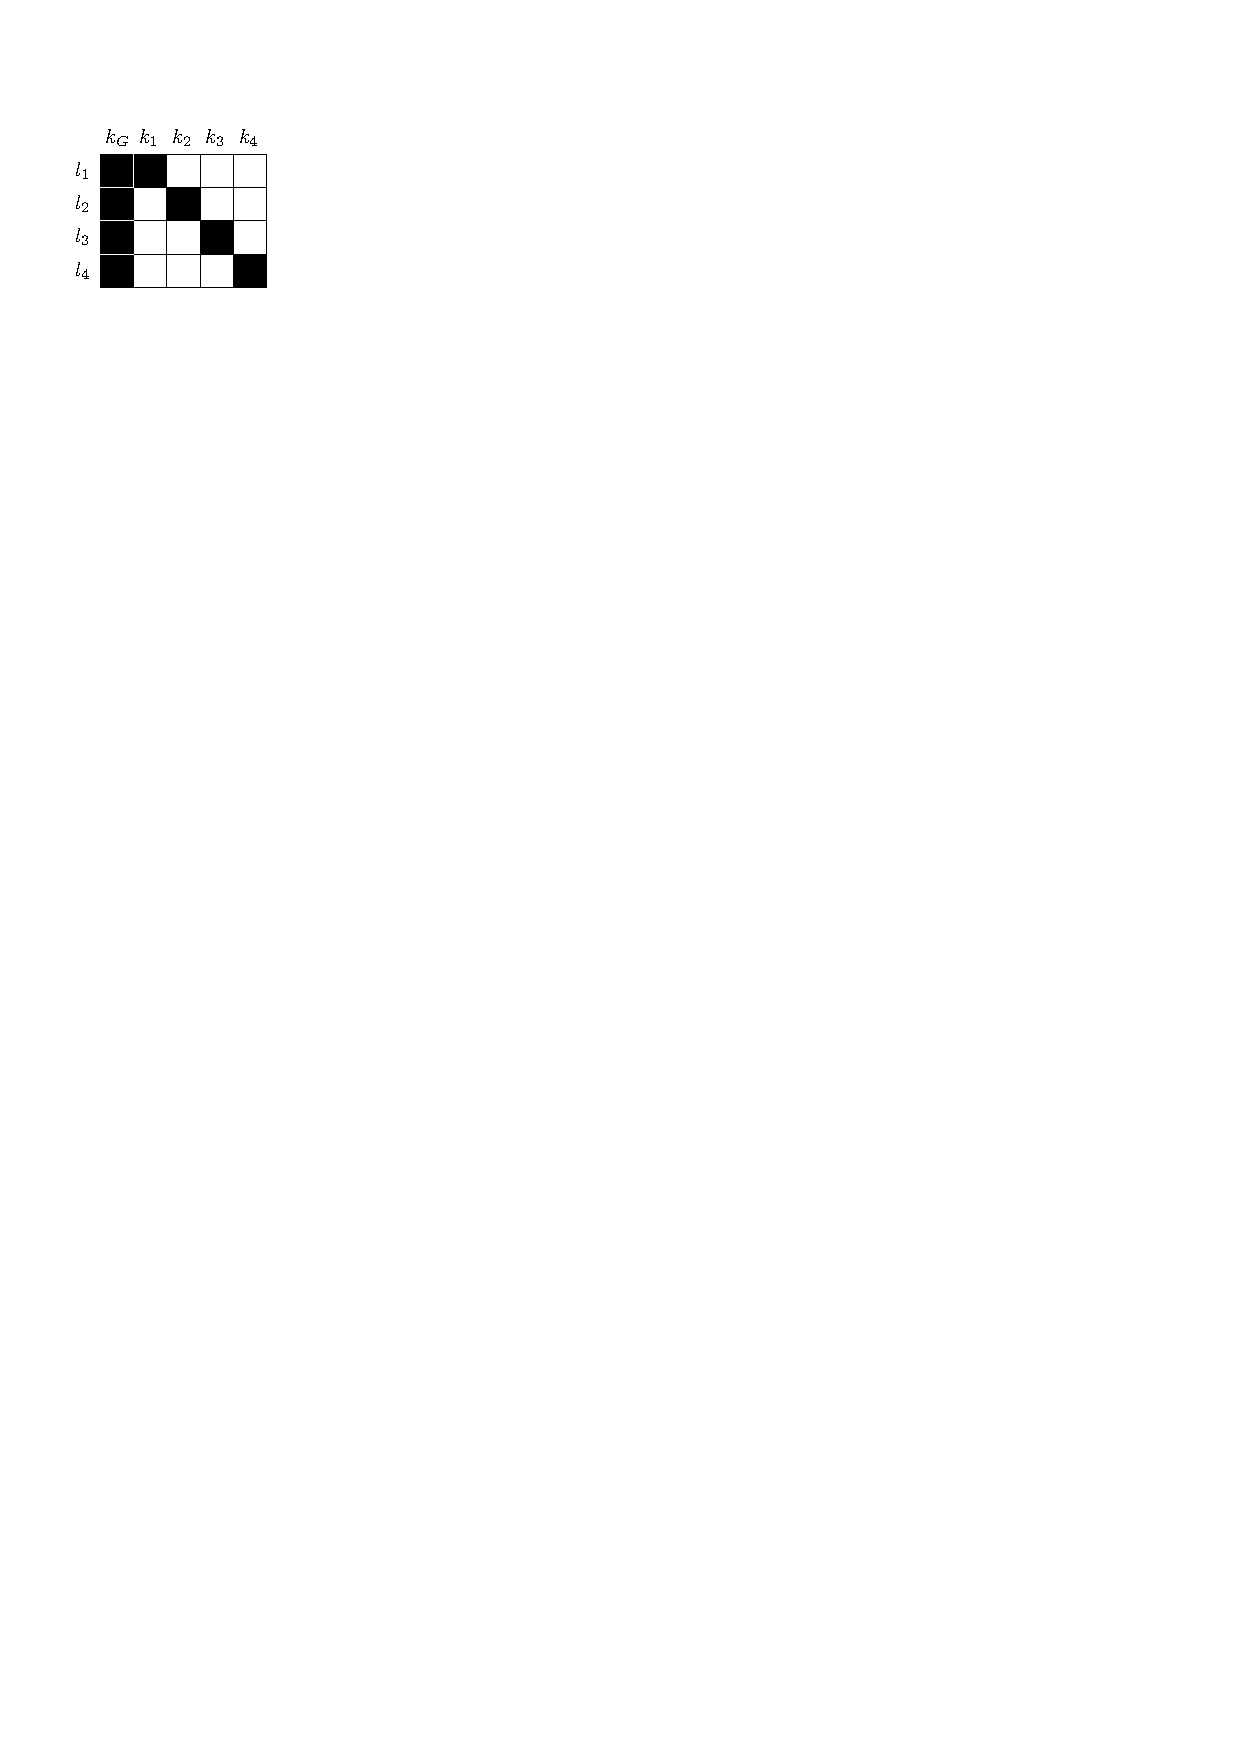
\includegraphics{DiagonalLockChart.pdf}
  \end{minipage}
  \hfill
  \begin{minipage}[t][180pt][t]{.63\textwidth}
    \begin{itemize}
      \item \textbf{Assumptions:}
      \begin{enumerate}
        \item The lock-chart is diagonal.
        \item Only individual keys will be added in future.
      \end{enumerate}
      \item \textbf{Consequences:}
      \begin{enumerate}
        \item Pick cuttings from $S_{\hat{q}}$.
        \item The extremal lock-chart can have
        at most $|S_{\hat{q}}|$ individual keys / locks.
      \end{enumerate}
    \end{itemize}
  \end{minipage}
\end{frame}


\begin{frame}{Independent master keys}
  \begin{columns}
    \begin{column}{.2\textwidth}
      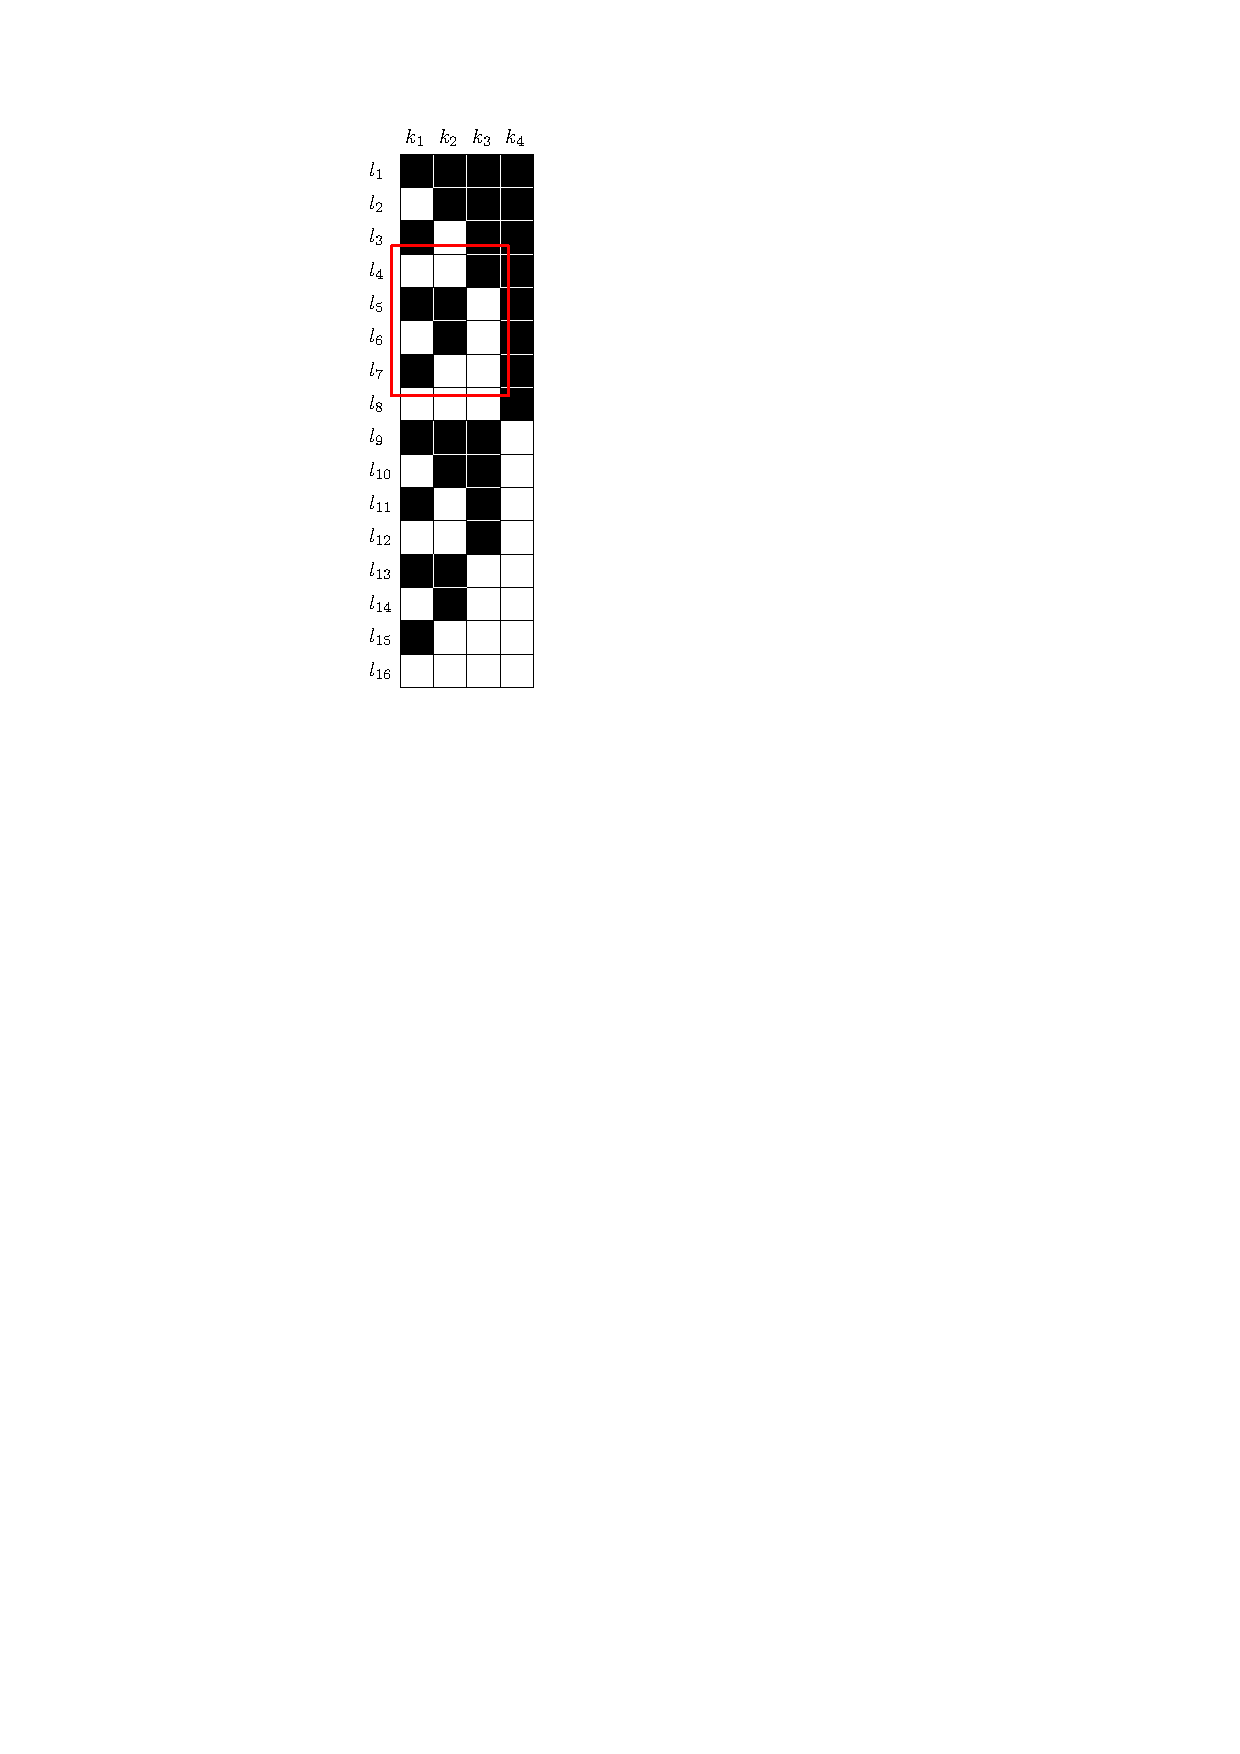
\includegraphics[height=0.8\textheight]{IndependentKeysLockChart.pdf}
    \end{column}

    \begin{column}{.8\textwidth}
      \begin{itemize}
        \item \textbf{Assumption:} Lock-chart has at most $p\cdot (d-1) + 1$ keys.
        \item \textbf{Consequences:}
        \begin{enumerate}
          \item Any lock can be added in future.
          \item There are $2^{p\cdot (d-1) + 1}$ such locks.
        \end{enumerate}
      \end{itemize}
    \end{column}
  \end{columns}
\end{frame}






\begin{frame}{Conclusions}
  \begin{itemize}
    \item The computational complexity proof show that the
    $\mathcal{P} \times \mathcal{NP}$ boundary disects the lock-chart problem.
    \item Practical cutting-counting algorithm allowed by the “compilation to gecons”.
    \item All-different pruning improves a state-of-the-art algorithm.
    \item SAT-based algorithm is the new baseline.
    \item Extensibility has been formalized.
  \end{itemize}
\end{frame}

\begin{frame}
  \begin{center}
    Thank you for your attention.
  \end{center}
\end{frame}



\begin{frame}{Question \#1}
  How many cylinders are there?

  \vfill

  \begin{itemize}
    \item Cutting is a $p$-dimensional vector
    with discrete values $\{1, \ldots, d\}$.
    There may be $d^p$ of them.
    \item On every position, a cylinder may or may not have a cutting depth $d$.
    There are $p\cdot d$ such binary choices. Together $2^{p\cdot d}$ cylinders.
  \end{itemize}
\end{frame}

\begin{frame}{Question \#2}
  \begin{block}{Citation}
    15 “real” constraint can be polynomially translated to gecons.  
  \end{block}

  \vfill

  \begin{block}{Reviewer's comment}
    For how many constraints is this true?
    Is there a common pattern among the remaining ones?
  \end{block}
  
  \vfill

  \begin{block}{Otázka oponenta}
    Pro kolik podmínek to je pravda
    a co měly společné podmínky,
    pro které to neplatilo?
  \end{block}

  \vfill
\end{frame}

\begin{frame}{Question \#3}
  All constraints that are translated to gecons,
  are translated to a polynomial number of gecons.

  \vfill

  \begin{block}{Example}
    “The first $n$ positions may not be equal.”

    \vfill

    Generates $\mathcal{O}(d \cdot n^2)$ gecons:
    \begin{tabular}{cccc}
      $(1,1,*,*,\ldots,*),$ & $(2,2,*,*,\ldots,*),$ & $\ldots,$ & $(d,d,*,*,\ldots,*)$ \\
      $(1,*,1,*,\ldots,*),$ & $(2,*,2,*,\ldots,*),$ & $\ldots,$ & $(d,*,d,*,\ldots,*)$ \\
      $(*,1,1,*,\ldots,*),$ & $(*,2,2,*,\ldots,*),$ & $\ldots,$ & $(*,d,d,*,\ldots,*)$ \\
      $\vdots$              & $\vdots$              & $\vdots$  & $\vdots$             \\
    \end{tabular}
  \end{block}
\end{frame}

\begin{frame}{Question \#3}
  Some constraints are not translatable to gecons.

  \vfill

  \begin{block}{Example}
    “Some two cutting depths differ by at least $n$.”
  \end{block}

  \vfill

  \begin{block}{Solution in the solver}
    We use \textit{existential constraints} (excons) \cite{horenovsky2018}.
    Used for constraints speaking about “existence” of a cutting depth.
  \end{block}
\end{frame}

\begin{frame}{Question \#4}

  \begin{block}{Reviewer's criticism}
    Theoretical results are straightforward,
    except for Theorem 52, whose proof is incomplete.
  \end{block}
  
  \vfill

  \begin{block}{Výhrada oponenta}
    K teoretickým výsledkům mám výhrady:
    jsou povětšinou přímočaré s výjímkou věty 52,
    která má neúplný důkaz.
  \end{block}
\end{frame}

\begin{frame}{Question \#4}
  \begin{itemize}
    \item Proofs in the theoretical results are straightforward indeed.
    \item Most of them fit within a single A5 page (see page 37).
    \item The results are still novel.
  \end{itemize}
\end{frame}

\begin{frame}{Question \#4}
  \begin{center}
    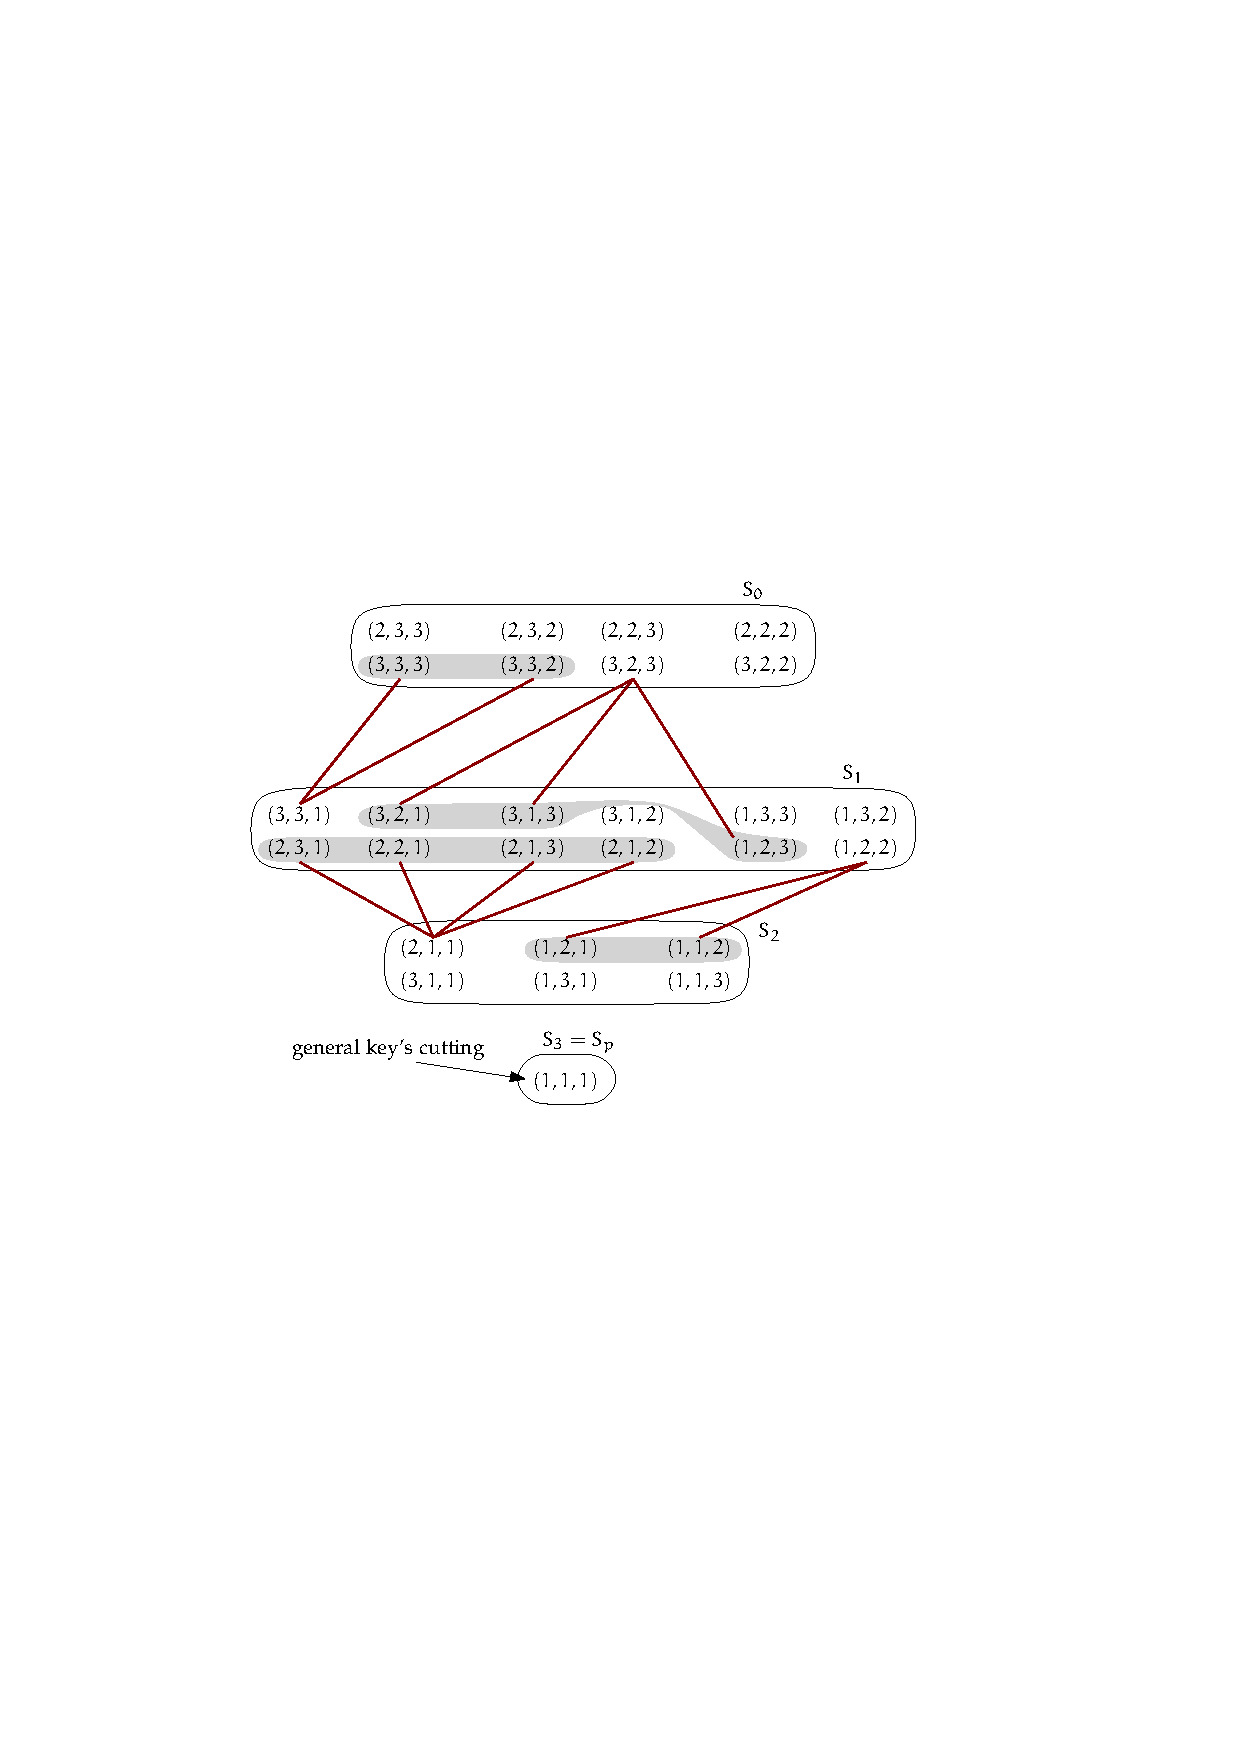
\includegraphics[height=0.8\textheight]{UpperBoundIllustration.pdf}
  \end{center}
\end{frame}

\begin{frame}{Question \#4}
    \begin{itemize}
      \item Let $0 \leq q < r \leq p$,
      $S_q' \subseteq S_q$, $S_r' \subseteq S_r$
      and $S_q' \cup S_r'$ be an independent set.
      \item Proved that $$|S_q'| + |S_r'| \leq \max\{|S_q|, |S_r|\}\ .$$
      \item Can $|S_q'| + |S_r'| + |S_s'| + \cdots \leq \max\{|S_q|, |S_r|, |S_s|, \ldots\}$?
      \pause
      \item Proof is incomplete.
      \item There is no known counter-example.
      \item I am convinced that the theorem still holds.
    \end{itemize}
\end{frame}

\begin{frame}{Question \#5}
  \begin{block}{Reviewer's comment}
    The algorithms were tested in the “vanilla framework”,
    but the gecons alone cause NP-completeness.
    Are there resons to believe that the results
    would not change [if gecons were included]?
  \end{block}
  
  \begin{block}{Otázka oponenta}
    Testování algoritmů proběhlo ve „vanilla framework“.
    Samotná omezení ve formě geconů zapřičiňují NP-úplnost.
    Existují důvody pro to, že by se výsledky podstatně nezměnily
    při porovnávání vstupních dat z praxe?
  \end{block}
\end{frame}

\begin{frame}{Question \#5}
  \begin{itemize}
    \item Let's assume that the Lawers' algorithm can (somehow) accomodate gecons.
    \item \textbf{Will SAT be still better?}
  \end{itemize}

  \pause
  \begin{enumerate}
    \item \textbf{Runtime}:
    \begin{itemize}
      \item Finding a valid key cutting given real-world constraints is easy ($\leq 1\,$ms).
      \item Gecons are applied to each key separately (exploited by DPLL).
      \item Finding valid key cuttings for $\sim 100$ keys is $\leq 1\,$s.
    \end{itemize}
    \pause
    \item \textbf{Criterial function:}
    \begin{itemize}
      \item Some modifications to the strategy are needed.
      \item It is tricky to pick a cutting depths to forbid.
      \item This is done in the commercial product.
      \item Lock-charts of size $\sim 25$ keys can still be optimized within $3\,$s.
    \end{itemize}
    \item Also, the 2 orders-of-magnitude margin is very big.
  \end{enumerate}
\end{frame}

\begin{frame}{Question \#0}
  \begin{block}{Reviewer's comment}
    Based on the presented research,
    has there been a progamme written
    that could be practically used
    to design master keyed systems?
  \end{block}
  \begin{block}{Otázka oponenta}
    Byl na základě představeného výzkumu napsán program,
    který se v praxi použil na návrh zámků a klíčů,
    případně na nějaké dílčí úlohy?
  \end{block}
\end{frame}

\begin{frame}{Question \#0}
  \begin{itemize}
    \item Yes.
    \item The translation to SAT is already in production.
    \item A fully fledged all-different pruning is in development.
  \end{itemize}
\end{frame}

\begin{frame}
  \bibliographystyle{humanbio}
  \bibliography{References}
\end{frame}
\end{document}
